\newcommand{\tb}[1]{\textcolor{blue}{#1}}
\definecolor{applegreen}{rgb}{0.05, 0.41, 0.0}
\newcommand{\tg}[1]{\textcolor{applegreen}{#1}}

\section*{Notation}

The following notation is used throughout the paper: the 2-norm for a function $f$ is denoted  by $\|f\|$ and for a vector $x\in\RR^n$ by $\|x\|$. 
The dual convex cone to a convex cone $K$ defined by
\begin{equation}
  \label{eq:dual-cone}
  K^\star = \{u \in \RR^3 \mid  r^\top u \geq 0, \quad \text{for all } r \in K   \}.
\end{equation}
\section{Introduction}


More than thirty years after the pioneering work of~\cite{Panagiotopoulos_IA1975},~\cite{Necas.ea1980},~\cite{Haslinger1983,Haslinger1984},\cite{Katona_IJNAMG1983},~\cite{Chaudhary.Bathe_CS1986},~\cite{Jean.Moreau1987},~\cite{Mitsopoulou.Doudoumis1988} on numerically solving mechanical problems with contact and friction, there are still active research activities on this subject in the computational mechanics and applied mathematics communities.  This can be explain by the fact that \tg{problems from} mechanical systems with unilateral contact and Coulomb friction are difficult to numerically solve and the mathematical results of convergence of the numerical algorithms are rare and most of these require rather strong assumptions. In this paper, we want to give some insights of the advantages and weaknesses of standard solvers found in the literature by comparing them on the large sets of examples coming from a wide range of mechanical systems.

\begin{ndroh}
 The following paragraph is too technical for the intro IMHO
\end{ndroh}
To fix ideas, we want to discuss possible numerical solution procedures for the following three--dimensional discrete frictional contact problem and some of its variants.  Let $n_c\in \NN$ be the number of contact points and $n\in\NN$ the number of degree of freedom of a discrete mechanical system.  \tb{For each contact $\alpha$, the unknown local variables  $u^\alpha\in\RR^3$ (relative velocity or gap at the contact point) and $r^\alpha\in\RR^3$ (reaction or impulse) are decomposed  in a contact local basis $({\sf N}^\alpha,{\sf T_1}^\alpha,{\sf T_2}^\alpha)$ such that $u^\alpha = u^\alpha_{\n} {\sf N}^\alpha +   u^{\alpha}_{\tone}{\sf T_1}^\alpha + u^{\alpha}_{\ttwo}{\sf T_2}^\alpha , u^\alpha_{\n} \in \RR, u^\alpha_{\t} = [u^{\alpha}_{\tone},u^{\alpha}_{\ttwo}]^\top \in \RR^2$ and  $r^\alpha = r^\alpha_{\n} {\sf N}^\alpha +   r^{\alpha}_{\tone}{\sf T_1}^\alpha + r^{\alpha}_{\ttwo}{\sf T_2}^\alpha  , r^\alpha_{\n} \in \RR, r^\alpha_{\t}=[r^{\alpha}_{\tone},r^{\alpha}_{\ttwo}]^\top \in \RR^2$ (see Figure~\ref{fig:local-frame}).}

 Given a symmetric positive (semi-) definite matrix ${M} \in \RR^{n \times n}$, a vector $ {f} \in \RR^n$, a matrix  ${H} \in \RR^{n \times m}$ with $m= 3n_c$, a vector $w \in \RR^{m}$ and a vector of coefficients of friction $\mu \in \RR^{n_c}$, find two vectors $ {v} \in \RR^n$ and $r\in \RR^m$ such that
\begin{equation}\label{eq:soccp1-intro}
  \begin{array}{rcl}
    M v = {H} {r} + {f}, &
    u = H^\top v + w,  &
    \hat u = u + g(u) ,\\[1mm]
    &    K^\star \ni {\hat u} \perp r \in K,&
  \end{array}
\end{equation}
where the set $K$ is the cartesian product of Coulomb's friction cone at each contact, that is
\begin{equation}
  \label{eq:CC}
  K = \prod_{\alpha=1\ldots n_c} K^{\alpha}  = \prod_{\alpha=1\ldots n_c} \{r^\alpha, \|r^\alpha_\t \| \leq \mu^\alpha |r^\alpha_\n| \}
\end{equation}
and $K^\star$ is dual. The function $g(u)$ is a nonsmooth function defined as
\begin{equation}
g(u) = [[\mu^\alpha  \|u^\alpha_\t\| {\sf N}^\alpha]^\top, \alpha = 1\ldots n_c]^\top\label{eq:gg}. 
\end{equation}\tb{The variable $u$ and $\hat u$  do not appear as unknowns since they can be directly obtained from $v$.}
\marginpar{\tg{missing end}}\tb{The vector is}
\begin{figure}
  \centering
  \begin{tikzpicture}[ scale=4,
      axis/.style={ ->, >=stealth'},
      normal/.style={ thick, ->, >=stealth'},
      important line/.style={very thick},
      dashed line/.style={dashed, thin},
      every node/.style={color=black},
      soldot/.style={only marks,mark=*},
      holdot/.style={fill=white,only marks,mark=*}
      ]
      % body
      \node (BodyA) at (1,-1) {Body A};
      \fill[gray!20] (1,0) arc (0:-90:1);
      \fill[gray!20] (1,0) arc (90:180:1);
      \draw (1,0) arc (90:180:1);

      \node (BodyB) at (-1,1) {Body B};
      \draw (0,1) arc (0:-90:1);
      \fill[gray!20] (0,1) arc (90:180:1);
      \fill[gray!20] (0,1) arc (0:-90:1);

      % local frame
      \def\nlength{0.35};
      \coordinate (CA)  at  ({1.0-sqrt(2)/2.0},{-1.0+sqrt(2)/2.0});
      \node[] at  (CA) [below] {$\sf C_A$};
      \draw[holdot]  (CA) circle(0.05em);
      \draw[normal] (CA) -- ($(CA)+({-\nlength*sqrt(2)/2.0},{+\nlength*sqrt(2)/2.0 })$) node [right] {$\,\sf N$};
      \draw[normal] (CA) -- ($(CA)+({-\nlength*sqrt(2)/2.0},{-\nlength*sqrt(2)/2.0 })$) node [above] {$\sf T_1\quad$};
      \draw[dashed line] (BodyA) -- (BodyB);
      \draw[holdot] ($(CA)+({\nlength*sqrt(3)/2.0},{0.0})$) circle(0.2em);
      \node at ($(CA)+({\nlength*sqrt(3)/2.0},{0.0})$) [right]{$\sf T_2$};
      \draw[soldot] ($(CA)+({\nlength*sqrt(3)/2.0},{0.0})$) circle(0.02em);

      \coordinate (CB)  at  ({-1.0+sqrt(2)/2.0},{1.0-sqrt(2)/2.0});
      \node at  (CB) [above] {$\sf C_B$};
      \draw[holdot]  (CB) circle(0.05em);

      \draw[axis] (CA) -- (CB) node[midway, below left ] {$\sf g_\n$} ;
      
      % \draw[axis] (0,-0.4) -- (0,0.4) node(yline)[right] {$\sgn(x)$};
      % % lines
      % \draw[important line] (-0.4,-0.3) -- (0.   ,-.3);
      % \draw[important line] (0.0,0.3) --(.4,.3)  ;
      % \coordinate (O) at (0.0, 0.05);
      % \draw[fill] (O) circle (0.03em);
      % \draw (0.0,0.05) node[right]{$a$};
      % \draw (0.0,0.3) node[left]{$1$};
      % \draw (0.0,-0.3) node[right]{$-1$};
      % \draw[holdot] (0.0,0.3) circle (0.03em);
      % \draw[holdot] (0.0,-.3) circle (0.03em);
    \end{tikzpicture}
\caption{Contact kinematic}
\label{fig:local-frame}
\end{figure}

We clearly choose to simplify a lot the general problems of formulating the contact problems with friction by avoiding including too much side effects that are themselves interesting but render the study too difficult to carry out in a single article. We choose finite dimensional systems where the time dependence does not appear explicitly. For instance, we consider systems that are discretized both in space and time if the original system is not a finite dimensional system and if a dynamic or a quasi--static evolution is considered. In the same way, we consider a linear setting in a first attempt and we assume that  nonlinear mechanical bulk behaviors that can be treated at an upper level with a Newton linearization procedure. Even under these assumptions, we believe that there are a strong interest to work on the problem since it appears to be relatively generic in numerous of simulations of systems with contact and friction. This problem is indeed at the heart of the simulation of mechanical systems with 3D Coulomb's friction and unilateral constraints: it might be the result of the time--discretization by event--capturing time--stepping methods or event--detecting (event--driven) techniques of dynamical systems with friction or the result of a space--discretization (by FEM for instance) of the quasi-static problems of frictional contact mechanics. For a description of the derivation of such problems in various practical situations we refer to~\cite{Acary.Brogliato2008,Acary.Cadoux2013}.{\tt XXX discuss the remark Olivier about the motion of this paragraph. }

From the mathematical programming point of view, the problem appears to be a Second Order Cone Complementarity Problem (SOCCP)~\cite{Facchinei.Pang2003} which can be generically defined as
\begin{equation}
  \begin{cases}
    y =f(x) \\
    K^\star \ni y \perp x \in K,
  \end{cases}
\end{equation}
where $K$ is a second order cone. If the nonlinear part of the problem~\eqref{eq:soccp1-intro} is neglected ($g(u)=0$), the problem is an associated friction problem with dilatation, and by the way, is a gentle Second Order Cone Linear Complementarity Problem (SOCLCP) with a positive definite matrix $H^\top M^{-1} H$ (possibly semi--definite).\tb{The assumption of associated frictional law, i.e, a friction law where the local sliding velocity is normal the friction cone differs dramatically from the standard Coulomb friction since it generates a non--vanishing normal velocity when we slide. In other terms, the sliding motion implies the separation of the bodies.}
When the non-associated character of the friction is taken into account through $g(u)$, the problem is non monotone and nonsmooth, and therefore is very hard to solve efficiently. For a given numerical algorithm, it is not so difficult to design mechanical example to run the algorithm into troubles.
\tg{Proof of convergence} of the numerical algorithms are rare and most of these required strong assumptions \tg{on either} the friction coefficients or full rank assumptions of matrices or operators or the dimension of the space in which the problem is formulated. Among these results, we can cite the Czech school where the coefficient of friction is assumed to be bounded and small. This assumption allows us to use fixed point methods on the convex sub--problems of Tresca friction \tb{(friction threshold that does depend on the normal reaction and then transform the cone into a semi-cylinder)}. We can also mention the results from~\cite{Pang.Trinkle1996,Stewart.Trinkle1996,Anitescu.Potra97} where the friction cone is polyhedral (in 2D or by a faceting process). In that case, if $w=0$ or $w \in \mathrm{im}(H^\top)$, Lemke's algorithm is able to solve the problem. The question of existence of solutions has been treated in~\cite{Klarbring.Pang1998,Acary.ea_ZAMM2011} under similar assumptions but with different techniques. The question of uniqueness remains a difficult problem in the general case.


In this article,  after stating the problem with more details in Section~\ref{sec:description}, we recall the existence result of~\cite{Acary.ea_ZAMM2011} for the problem in~\eqref{eq:soccp1-intro} in Section \ref{sec:existence}. In this framework, we briefly present in Section~\ref{sec:formulation} \tg{a few} alternative formulations of the problem that enable the design of numerical solution procedures. Right after these formulations, we list some of the most standard algorithms dedicated to one of the previous formulation in Sections~\ref{sec:numericalmethods,vi},~\ref{sec:newtonmethods},~\ref{Sec:SplittingTechniquesAndProx}, \ref{Sec:InteriorPoint} and \ref{Sec:OptimisationBasedMethods}. These algorithms that have been previously developed for solving the SOCCP~\eqref{eq:soccp1-intro} are mainly based on  variational inequality (Section~\ref{sec:numericalmethods,vi} and~\ref{Sec:SplittingTechniquesAndProx}) or nonsmooth equations (Section~\ref{sec:newtonmethods}) or  optimization--based (Section~\ref{Sec:OptimisationBasedMethods}) reformulations.  

Since it is difficult to be exhaustive on the approaches developed in the literature to solve frictional contact problems, we decided to leave out the scope of the paper the following approaches:
\begin{itemize}
\item the approaches that alter the fundamental assumptions of the 3D Coulomb friction model by faceting the cone as in the pioneering work of~\cite{Klarbring1986} and followed by~\cite{AlFahed.Stavroulakis.ea1991,Pang.Trinkle1996,Stewart.Trinkle1996,Anitescu.Potra97,Haslinger.ea_JCAM2004}, or by convexifying the Coulomb law (associated friction law with normal dilatancy)~\cite{Heyn.ea_IJNME2013,Tasora.Anistescu_Meccanica2013,Tasora.Anistescu_CMAME2011,Anistescu.Tasora_COA2010,Tasora.Anistescu_CMAME2009} or finally by regularizing the friction law~\cite{Kikuchi.Oden_SIAM1988}.
\item Approaches that not give satisfactory results
\item Approaches that we have not yet implemented. 
  \begin{enumerate}
  \item \item Interior point.
    
    \cite{Kleinert.ea_CMAME2014} and references therein
    
    \cite{Christensen.Pang1998}
    
    \cite{Heyn.ea_IJNME2013} + PhD thesis~\cite{Heyn_PhD2013}
    
    Frictionless?~\cite{Miyamura.ea_IJNME2010,Temizer.ea_CMAME2014}
 
  \item SOCCP Solver ??
  \end{enumerate}
\textcolor{pink}{\item Approaches based on domain decomposition and parallel computing. (cite a bit a literature Krause, Koziara, Renouf, Heyn, .... )}
\end{itemize}

Other comparisons articles have already been published in the literature. Cite and comment

\begin{list}{}{}
\item~\cite{Raous.ea1988,Chabrand.ea_MCM1998}
\item~\cite{Christensen.Klarbring.ea1998}
\item~\cite{Mijar.Arora_SMO2000,Mijar.Arora_ACME2000,Mirar.Arora_SMO2004-I,Mirar.Arora_SMO2004-II}
\end{list}


The comparison are performed on a large set of examples using performance profiles.
\tg{Let us summarize the main conclusion from Section~\ref{sec:numericalcomparisons}:
on one hand}, the algorithms based on Newton methods for nonsmooth equations solve quickly the problem when they succeed, but suffer from robustness issues mainly if the matrix $H$ has not full rank. On the other hand, the
iterative methods dedicated to solving variational inequalities are quite robust but with an extremely slow rate of convergence. To sum up, as far as we know there is no option that combines time efficiency and robustness.
\tg{The set of problems used here are from the FCLIB collection\footnote{\url{http://fclib.gforge.inria.fr}}, which aims at providing many problems to compare algorithms on a fair basis}.  In this work, this collection is solved with the software {\sc Siconos} and its component {\sc Siconos/Numerics}\footnote{\url{http://siconos.gforge.inria.fr}}\citep{Acary.Bremond.Huber.Perignon2015}.


\clearpage
\section{Description of the 3D frictional contact problems}
\label{sec:description}
\subsection{Signorini's condition and Coulomb's friction.}

Let us consider the contact between two  bodies $A \subset  \R^3$ and $B \subset \R^3$ with sufficiently smooth boundaries, \tg{as depicted on} Figure~\ref{fig:local-frame}.
\tg{From the body $A$ ``perspective'', the point $C_{A} \in \partial A$ is called a \emph{master point to contact}}.  The choice of this master point $C_A$ to write the contact condition is crucial in  practice and amounts to consistently discretizing  the contact surface. The vector  ${\sf N}$ defines an outward unit normal vector to $A$ at the point $C_A$. With $\sf T_1, T_2$ two vectors in the plane orthogonal to ${\sf N}$, we can build  an orthornormal frame $(C_A, \sf N, T_1, T_2)$ called the \emph{local frame at contact}. The slave contact point $C_B \in \partial B$ is defined as the projection of the point $C_A$ on $\partial B$ in the direction given by $\sf N$. Note that we assume that such a point exists. The gap function is defined as the signed distance between $C_A$ and $C_B$
\begin{equation}
  \label{eq:gap}
  g_{\n} = (C_B-C_A)^\top  \sf N.
\end{equation}


To fix ideas, if we consider two strictly convex bodies, which are non penetrating, {\it i.e.}  $A \cap B = \emptyset$, the master and slave contact points can be chosen as the proximal points of each bodies and the normal vector  ${\sf N}$ can be written as
\begin{equation}
  \label{eq:normal}
  {\sf N} = \Frac{C_B-C_A}{\|C_B-C_A\|}.
\end{equation}
%
The contact force exerted by $A$ on $B$ is denoted by $r \in \RR^3$ and is decomposed in the local frame as
\begin{equation}
  \label{eq:reaction}
  r = r_{\n} {\sf N} +   r_{\tone}{\sf T_1} + r_{\ttwo}{\sf T_2}  ,\quad \text{ with  } r_{\n} \in \RR, r_{\t}=[r_{\tone},r_{\ttwo}]^\top \in \RR^2.
\end{equation}
%
The \emph{Signorini condition} states that
\begin{equation}
  \label{eq:signo}
  0 \leq g_{\n} \perp r_\n \geq 0,
\end{equation}
and models the unilateral contact. The condition~\eqref{eq:signo}, written at the \emph{position level}, can also be defined at the \emph{velocity level}.
\tg{To this end}, the relative velocity $u \in \RR^3$ of the point $C_{B}$ with respect to $C_{A}$ is also decomposed in the local frame
\begin{equation}
  \label{eq:velocity}
  u =  u_\n {\sf N} +  u_{\tone}{\sf T_1} + u_{\ttwo}{\sf T_2}  \quad \text{ with } u_\n \in \RR \text{ and } u_\t=[u_{\tone},u_{\ttwo}]^\top  \in \RR^2.
\end{equation}
\tg{At} the velocity level, the Signorini condition is written 
\begin{equation}
  \label{eq:signo-velocity}
  \left\{\begin{array}{ll}
  0 \leq u_{\n} \perp r_\n \geq 0  &\text{ if } g_{\n} \leq 0 \\
  r_{\n} =0 &\text{ otherwise}.
\end{array}\right.
\end{equation}
The Moreau's viability Lemma~\cite{Moreau1988} ensures that~\eqref{eq:signo-velocity} implies~\eqref{eq:signo} if $g_{\n}\geq 0$ holds in the initial configuration.

Coulomb's friction  models the frictional behavior of the contact force law in the tangent plane \tb{ spanned by $(T_1,T_2)$}. Let us define the Coulomb friction  cone $K$ which is chosen as the isotropic second order cone (Lorentz or ice--cream cone)
\begin{equation}
  \label{eq:CoulombCone}
  K = \{r \in \RR^3 \mid \|r_\t\| \leq \mu r_n\},
\end{equation}
where $\mu$ is the coefficient of friction. The Coulomb friction  states for the sticking case that 
\begin{equation}
  \label{eq:Coulom-stick}
  u_{\t} =0,\quad r \in K
\end{equation}
and for the sliding case that
\begin{equation}
  \label{eq:Coulom-slide}
  u_{\t}  \neq 0,\quad r \in \partial K, \exists\, \alpha > 0, r_\t = -\alpha u_\t.
\end{equation}
\tb{With the Coulomb friction model, there are two relations between $u_\t$ and $r_\t$. The distinction is based on the value of the relative velocity $u_\t$ between the two bodies. If $u_\t=0$ (sticking case), we have $r_\t \leq \mu r_n$. On the other hand, we get the sliding case.} 
\marginpar{\tg{takeoff case?}}
\paragraph{Disjunctive formulation of the Signorini-Coulomb model}

If we consider the velocity-level Signorini condition~\eqref{eq:signo-velocity} together with the Coulomb friction~\eqref{eq:Coulom-stick}--\eqref{eq:Coulom-slide} which is naturally expressed in terms of velocity, we obtain a disjunctive formulation of the frictional contact behavior as
\begin{equation}
  \label{eq:contact-disjunctive}
  \left\{\begin{array}{llr}
      r = 0  &\text{ if } g_{\n} > 0  & \text{(no contact)}\\
      r = 0,  u_\n \geq 0   &\text{ if } g_{\n} \leq 0 & \text{(take--off)} \\
      r \in K, u =0 &\text{ if } g_{\n} \leq 0 & \text{(sticking)}  \\
      r \in \partial K,u _\n=0,  \exists\,\alpha > 0, u_\t = -\alpha r_\t &\text{ if } g_{\n} \leq 0 & \text{(sliding)}  \\
\end{array}\right.
\end{equation}
In the computational practice, the disjunctive formulation is not suitable for  solving the Coulomb problem as it suggests the use of enumerative solvers, with exponential behavior.
In the sequel, alternative formulations of the Signorini-Coulomb model \tg{suitable for} numerical applications are delineated.
\tg{The core idea is to translate the cases in~\eqref{eq:contact-disjunctive} into complementarity relations.}

\paragraph{Inclusion into normal cones} The Signorini condition~\eqref{eq:signo} in their complementarity forms can be equivalently written  as an inclusion into a normal cone to $\RR_+$
\begin{equation}
  \label{eq:signo-inclusion}
  - g_\n \in N_{\RR_+}(r_\n),
\end{equation}
and respectively for~\eqref{eq:signo-velocity}
\begin{equation}
  \label{eq:signo-inclusion-velo}
  - u_\n \in N_{\RR_+}(r_\n),
\end{equation}
if $g_{\n} \leq 0$ and $r_\n =0 $ otherwise. An inclusion form of the Coulomb friction can be also proposed introducing the Coulomb disk $D(\mu r_n)$
\begin{equation}
  \label{eq:diskR}
  D(\mu r_\n) = \{r_\t \in \RR^2\mid \|r_T\| \leq \mu r_\n   \}.
\end{equation}
For the Coulomb friction, we get
\begin{equation}
  \label{eq:Coulomb-inclusion}
  - u_{\t} \in N_{D(\mu r_\n)}.
\end{equation}
Since $D(\mu r_\n)$ is not a cone, the inclusion~\eqref{eq:Coulomb-inclusion} is not a complementarity problem.  The formulation~\eqref{eq:Coulomb-inclusion} is often related to Moreau's maximum dissipation principle of the frictional behavior,
\begin{equation}
  \label{eq:moreau-maxprinciple}
  r_\t \in \argmax_{\|z\| \leq \mu r_n}\;  z^\top u_\t.
\end{equation}
This means that the couple $(r_\t,u_\t)$ maximizes the energy lost through dissipation.


\paragraph{SOCCP formulation of the Signorini-Coulomb model}

In~\cite{Acary.Brogliato2008,Acary.ea_ZAMM2011}, another formulation is proposed inspired by the so-called bipotential~\cite{DeSaxce92,DeSaxce.Feng90,DeSaxce.Feng_MCM1998}.
\tg{The goal is to form a complementarity problem out of~\eqref{eq:signo-inclusion-velo} and~\eqref{eq:Coulomb-inclusion}}
To this end, we introduce the modified relative velocity $\hat u \in \RR^3$ defined by
\begin{equation}
  \label{eq:modified-velocity}
  \hat u = u +\mu \|u_\t\| \sf N.
\end{equation}
The entire contact model~\eqref{eq:contact-disjunctive} can be put into a Second-Order Cone Complementarity Problem (SOCCP) as
\begin{equation}
  \label{eq:contact-SOCCP}
 K^\star \ni \hat u \perp r \in K
\end{equation}
 if $ g_\n \leq 0 $ and $r=0$ otherwise. 
\begin{figure}\centering
  \resizebox{!}{0.5\textheight}{\input{../figure/cone1-b.pdf_t}}
  \caption{Coulomb's friction law in the sliding case.}
\label{fig:CoulombLawSliding}
\end{figure}

% \begin{tikzpicture}
%   % \tkzCone{3}{0.5}{5};\hspace{4cm}
%   % \tkzCone{5}{1.0}{5};\hspace{4cm}
%    \tkzCone{3}{2.0}{8};\hspace{4cm}
%   %\tkzCone{5}{0.1}{5};
% \end{tikzpicture}



\subsection{Frictional contact discrete problems}

In this section, we formulate two basic discrete frictional contact problems considering a finite number $n$ of degrees of freedom  together with a discrete linear dynamics.
\tb{ The first problem is directly related to~\eqref{eq:soccp1-intro} and keep the unknown triplet $(v,u,r)$.
The second problem will assume that the matrix $M$ is invertible. In that later case, we case eliminate the variable $v$ and reduce the unknown to the couple $(u,r)$.}

 We assume that a finite set of $n_c$ contact points and their associated local frames has been defined.
 In general, this task is not straightforward and amounts to correctly discretizing  the contact surfaces. For more details, we refer to~\cite{Wriggers2006,Laursen2003}.

For each contact $\alpha \in \{1,\ldots n_c\}$, the  local velocity  is denoted by $u \in \RR^3$, the normal velocity by $u_\n^{\alpha}\in \RR$ and the tangential velocity by $u_\t^\alpha\in\RR^2$. One obviously 
gets
\begin{equation}
  \label{eq:contactvelocity}
  u^\alpha =\left[
  \begin{array}{c}
    u^\alpha_{\n} \\
    u^\alpha_{\t}   
  \end{array}\right].
\end{equation}
The vector $u, u_\n, u_\t$ respectively collects all the local velocity
$  u = [[u^\alpha]^\top, \alpha = 1\ldots n_c]^\top$,
all the normal velocity 
$
  u_\n = [ u^\alpha_{\n}, \alpha = 1\ldots n_c]^\top$,
and all the  tangential velocity
$
  u_\t = [ [u^\alpha_{\t}]^\top, \alpha = 1\ldots n_c]^\top$.
For a contact $\alpha $, the modified local velocity, denoted by $\hat u^\alpha $, is defined by
\begin{equation}
  \label{eq:modified}
  \hat u^\alpha = u^\alpha + g^\alpha(u)
\end{equation}
where
\begin{equation}
  \label{eq:modified-bis}
  g^\alpha(u) =  \mu^\alpha  \|u^\alpha_\t\| {\sf N}^\alpha.
\end{equation}
The vectors $\hat u$ and $g(u)$ collect all the modified local velocity at each contact $\hat u = [[\hat u^\alpha]^\top, \alpha = 1\ldots n_c]^\top$ and the function $g(u) = [[\mu^\alpha  \|u^\alpha_\t\| {\sf N}^\alpha]^\top, \alpha = 1\ldots n_c]^\top$.

% Let us introduce finally the following notation to express the function $g(u)$ conveniently. We denoted by $s^\alpha = \|u^\alpha_\t\|$ the norm of the sliding velocity for the contact $\alpha$. The vector $s$ collects all the sliding velocity at each contact $s = [ s^\alpha, \alpha = 1\ldots n_c]^\top$. The matrix $ N \in \RR^{3n_c\times n_c}$ is composed of the vector $ mu^\alpha N^\alpha$ on its diagonal formally $N = \mbox{diag}(\mu^\alpha N^\alpha$. The function $g()$ can be therefore expressed as $g(u) = N s$.

For each contact $\alpha$, the reaction vector $r^\alpha\in \RR^3$ is also decomposed in its normal part $r_\n^{\alpha}\in \RR$ and the tangential part $r_\t^\alpha\in\RR^2$ as
\begin{equation}
  \label{eq:contactreaction}
  r^\alpha = \left[
  \begin{array}{c}
    r^\alpha_{\n} \\
    r^\alpha_{\t}   
  \end{array}\right].
\end{equation}
The Coulomb friction cone for a  contact $\alpha$ is defined by $K^{\alpha}  = \{r^\alpha, \|r^\alpha_\t \| \leq \mu^\alpha |r^\alpha_\n| \}$ and the set $K^{\alpha,\star}$ is its dual. 
The set $K$ is the cartesian product of Coulomb's friction cone at each contact, that is
\begin{equation}
  \label{eq:CC_bis}
  K = \prod_{\alpha=1,\ldots,n_c} K^{\alpha}\quad\text{and}\quad K^\star\;\text{is its dual.}
\end{equation}
In this paper, we investigate the case where the problem is given in its \emph{reduced} form.
We consider that the discretized dynamics are of the form
\begin{equation}
 M v = {H} {r} + {f},
 \label{eq:global_dyn}
\end{equation}
with $M$ an symmetric positive-definite matrix. The local velocities at the point of contact are given by
\begin{equation}
  u = H^\top v + w.
  \label{eq:local_v}
\end{equation}
More information on the term $w$ is given later in this section.
The (global) velocities $v$ can be substitute in~\eqref{eq:local_v} by using a Schur-complement technique.
This yields
\begin{equation}
u = H^\top M^{-1} H r + H^\top M^{-1} f +w.
\end{equation}
Let us define $W$, often called the \emph{Delassus matrix}, as
\begin{align}
  \label{eq:Delassus}
  W&\coloneqq H^\top M^{-1} H 
\intertext{and the vector $q$ as}
  \label{eq:qq}
  q&\coloneqq H^\top M^{-1} f + w.
\end{align}

\begin{problem}[Discrete frictional contact problem]\label{prob:II}
  Given
  \begin{itemize}
    \item a symmetric positive semi--definite  matrix ${W} \in \nbR^{m \times m}$,
    \item a vector $ {q} \in \nbR^m$,
    \item a vector $\mu \in \RR^{n_c}$ of coefficients of friction, 
  \end{itemize}
find  a vector $r\in \RR^m$, denoted by $\mathrm{FC}(W,q,\mu)$  such that
\begin{equation}\label{eq:soccp2}
  \begin{cases}
    u =Wr +q \\[2mm]
    \hat u =u + g(u) \\[2mm]
    K^\star \ni {\hat u} \perp r \in K
  \end{cases}
\end{equation}
with $g(u) = [[\mu^\alpha  \|u^\alpha_\t\| {\sf N}^\alpha]^\top, \alpha = 1\ldots n_c]^\top$.
\qed
\end{problem}

%The  first two lines of~\eqref{eq:soccp1} may represent a linear time--discretized dynamics and $v$ have the role of the global or generalized velocity. 


%We will see in the next section how these systems can be  obtained and how they may also be an instance of a quasi-static problem
% Nonlinear versions of this problem can also be stated but they are out pf the scope of the paper. When the dynamics is nonlinear, an outer Newton linearization is performed leading to a linearized problem. 


\subsection{Existence of solutions}
\label{sec:existence}

The question of the existence of solution for the Problem~\ref{prob:II} have been studied in~\cite{Klarbring.Pang1998} and~\cite{Acary.ea_ZAMM2011} with different analysis techniques.
The key assumption for existence of solutions in both papers is as follows
\begin{equation}\label{ass}
   \exists v\in \RR^m \,:\: H^\top v + w \in \mathrm{int}\, K^\star,
\end{equation}
or equivalently
\begin{equation}\label{asseq}
  w\in\mathrm{im}\, H + \mathrm{int}\, K^\star.
\end{equation}
Under the assumption, the Problem~\ref{prob:II} have a solution. The question to provide a solution procedure to compute has therefore a sense. In the sequel, we will compare numerical methods only when this assumption is satisfied.

This assumption is easy verified in numerous applications. For applications in nonsmooth dynamics where the unknown $v$ is a relative contact velocity, the term $w$ vanishes if we have only scleronomic constraints. For $w \in \mathrm{im}(H^\top)$ (and especially $w=0$), the assumption is trivially satisfied. As it is explained in~\cite{Acary.Cadoux2013}, the term $w$ has several possible sources. \tb{If the constraints are written at the velocity level, one is given in dynamics by the impact law and in that case, we can show that of the Newton impact law it holds that $w \in \mathrm{im}(H^\top)$.   For other impact law, this is not so clear. Another source for $w$ is given by constraints that depends explicitly on time. In that case, we can have $w \not\in \mathrm{im}(H^\top)$ and non existence of solutions. If the constraints are written at the position level, $w$ can be given by initial of terms that comes velocity discretization. In that cases, the existence is not clear.}

\tb{The assumption is also satisfied if $\mathrm{im}\, H = \RR^m$ or in other words if $H^\top$ has full row rank. Unfortunately, in large number of applications $H^\top$ is rank deficient. }
From the mechanical point of view, the rank deficiency of $H$ and the amount of friction seems to play a fundamental role in the question of the existence (and uniqueness) of solutions. In the numerical comparisons, we will attempt to get a deeper understanding on the role of these assumptions on the convergence of the algorithms. The rank deficiency  of $H$ is related to the number of constraints that are imposed to the system with respect to the number of degree of freedom in the system. It is closely related to the concept of hyperstaticity in overconstrained systems. In the most favorable cases, it yields  indeterminate Lagrange multipliers but also to unfeasible problems and then to the lost of solutions in the worth cases. The second assumption on the amount of friction is also well--know. The frictionless problem is  easy to solve if it is  feasible. It is clear that large friction coefficients prevent from sliding and the therefore increase the degree of hyperstaticity of the system. 



% \subsection{Origins of the discrete problem}

% \begin{ndrva}
%   Is it mandatory ?
% \end{ndrva}


% \subsubsection{Finite freedom mechanics}



% \subsubsection{Quasi-static frictional contact problem}

%~\cite{Haslinger1983,Christensen.Klarbring.ea1998,Klarbring.Pang1999}

% \subsubsection{Dynamic frictional contact problem}

%~\cite{Moreau1998,Moreau1994,Moreau1999}

\clearpage
%----------------------------------------------------------------------------------%
\section{Alternative formulations}
%----------------------------------------------------------------------------------%
\label{sec:formulation}
In this section, various equivalent formulations of Problem~\ref{prob:II} are \tg{given.
Our goal is to show that} such problems can be recast into several well-known problems in the mathematical programming and optimization community.
These formulations will serve as a basis for numerical solution procedures that we develop in further sections.

\subsection{Variational Inequalities (VI) formulations}

Let us recall the definition a finite-dimensional $\mathrm{VI}(X,F)$: find $z\in X$ such that 
\begin{equation}
  \label{eq:vi}
  F^\top(z)(y-z) \geq 0 \quad\text{for all}\; y \in X,
\end{equation}
with $X$ a nonempty subset of $\RR^n$ and $F$ a mapping from $\RR^n$ into itself. We refer to~\cite{Harker.Pang1990,Facchinei.Pang2003} for the standard  theory of finite--dimensional variational inequalities. The easiest way to state equivalent VI formulations of Problem~\ref{prob:II} is to use the following equivalences:
\begin{equation}
  \label{eq:SOCCP-1}
  K^\star \ni {\hat u} \perp r \in K \quad\Longleftrightarrow\quad
  - {\hat u} \in N_K(r) \quad \Longleftrightarrow\quad \hat u^\top (s -r) \geq 0, \text{ for all } s \in K.
\end{equation}
For Problem~\ref{prob:II}, the following equivalent formulation in VI is directly obtained from
\begin{equation}
  \label{eq:inclusion-1}
  -(W r + q + g(Wr+q))  \in N_K(r).
\end{equation}
 The resulting VI is denoted by $\mathrm{VI}(F_{\vitwo},X_{\vitwo})$ with
\begin{equation}
  \label{eq:vi-II}
  F_{\vitwo}(r) \coloneqq W r +q + g(Wr+q)\quad\text{and}\quad X_{\vitwo} \coloneqq K.
\end{equation}

\paragraph{\tg{Uniqueness} properties.} 
%Concerning the mathematical properties of the obtained VI formulations, it is difficult to provide a general result of existence and uniqueness of solutions.
\tg{In the general case, it is difficult to prove uniqueness of solutions to~\eqref{eq:vi-II}.}
\tg{If we suppose that} the matrix $H$ has full rank and that friction coefficients are ``small'', a classical argument for the uniqueness of solution of VIs can be satisfied.
\tg{Note that the full rank hypothesis on $H$ implies that $W$ is positive. Therefore,} we have  $(x-y)^\top W (x-y) \geq C_W \|x-y\|^2$ with  $C_W>0$.
Using this relation in~\eqref{eq:vi-II} yields
\begin{equation}
  \label{eq:mono-II}
  \begin{array}{rcl}
    (F_{\vitwo}(x)-F_{\vitwo}(y))^\top(x-y) &=& (x-y)^\top W (x-y)  \\
    &  & \quad\quad + \sum _{\alpha =1}^{n_c} \mu^\alpha (x^\alpha_\n-y^\alpha_\n) [\|[Wx+q]^\alpha_\t \| - \|[Wy+q]^\alpha_\t \|] \\
    & \geq & C_W \|x-y\|^2  + \sum _{\alpha =1}^{n_c} \mu^\alpha (x^\alpha_\n-y^\alpha_\n) [\|[Wx+q]^\alpha_\t \| - \|[Wy+q]^\alpha_\t \|].
  \end{array}
\end{equation}
\tg{Note that} for small values of the coefficients of friction, the mapping $F_\vitwo$ is strictly monotone and this ensures that the VI has at most one solution~\citep[Theorem 2.3.3]{Facchinei.Pang2003}. The fact that $H$ is full rank also implies that the Assumption~\eqref{ass} for the existence of solutions is trivially satisfied. \tg{Hence,} there exists a unique solution to the $\mathrm{VI}(F_{\vitwo},X_{\vitwo})$.



\begin{ndrva}
  Use of homotopy (Haslinger ?)
\end{ndrva}

\subsection{Quasi-Variational Inequalities (QVI)}

\tg{Let us recast Problem~\ref{prob:II} into the QVI framework. A QVI is a generalization of the VI, where the feasible set is allowed to depend on the solution. Let us define this precisely:}
let $X$ be a multi-valued mapping  $\nbR^{n} \rightsquigarrow  \nbR^{n}$ and let  $F$ be a mapping from $\nbR^n$ into itself. The  quasi-variational inequality  problem, denoted by $\mathrm{QVI}(X,F)$ is to find a vector $z\in X(z)$ such that 
\begin{equation}
 \label{eq:qvi}
 F^{\top}(z) (y-z) \ge 0, \, \forall y \in X(z).
\end{equation}
The QVI formulations of the frictional contact problems are obtained by considering the inclusions~\eqref{eq:signo-inclusion-velo} and~\eqref{eq:Coulomb-inclusion}. We get 
\begin{equation}
  \label{eq:qvi-1}
  u^\top (s - r) \geq 0, \text{ for all } s \in C(\mu, r_\n),
\end{equation}
where $C(\mu, r_\n)$ is the Cartesian product of the semi--cylinders of radius $\mu^\alpha r_n^\alpha$ defined as
\begin{equation}
  \label{eq:cylinder}
  C(\mu, r_\n) \coloneqq \prod_{\alpha =1}^{n_c}\: \left\{ s \in \RR^3 \mid  s_\n \geq 0, \|s_\t\| \leq \mu^\alpha r^\alpha_n\right\}.
\end{equation}
Note that the QVI~\eqref{eq:qvi-1} involves only $u$ and not $\hat u$: this is the main interest of this formulation. The price to pay is the dependence on $r$ of the set $C(\mu,r_\n)$.
Problem~\ref{prob:II} can be expressed as a QVI by substituting the expression of $u$, which yields
\begin{equation}
  \label{eq:qvi-IIbis}
   (Wr+q)^\top (s - r) \geq 0, \text{ for all } s \in C(\mu,r_\n).
\end{equation}
\tg{This expression is compactly rewritten as} $\mathrm{QVI}(F_{\qvitwo},X_{\qvitwo})$, with 
\begin{equation}
  \label{eq:qvi-II}
  F_{\qvitwo}(r) \coloneqq  Wr+q \quad\text{and}\quad X_{\qvitwo}(r) \coloneqq C(\mu,r_\n) .
\end{equation}
Since $W$ is assumed to be positive semi-definite matrix, $F_{\qvitwo}$ is monotone. Thus we get an affine monotone $\mathrm{QVI}(F_{\qvitwo},X_{\qvitwo})$ for Problem~\ref{prob:II}.


\subsection{Nonsmooth Equations}
\label{Sec:NonsmoothEquations}

In this section, we reformulate of Problems\ref{prob:II} as an \tg{equation, as opposed to inclusion}.
\tg{The term nonsmooth equation highlights that the mapping we consider fails to be differentiable.}

More precisely for Problem~\ref{prob:II}, we search for an equation of the type
\begin{equation}
  \label{eq:ne-1}
  G(v,u,r) = 0
\end{equation}
where $G$ is generally \tg{only} locally Lipschitz continuous such that the zeroes $(u,v,r)$ of~\eqref{eq:ne-1} are the solutions of~\eqref{eq:soccp2}.
\tg{Several numerical methods can be used to solve such a nonsmooth equation}, ranging from fixed point algorithms to Newton's method.

\paragraph{Natural and normal maps for the VI formulations}

A first way to obtain some formulations based on nonsmooth equations of the frictional contact problems is to use the normal and natural maps, see~\cite{Facchinei.Pang2003} for details.
\tg{Those two mapping enable us} to restate a VI as a system of nonlinear and  nonsmooth functions.
\tg{Firstly,} let us define the Euclidean projector $P_X$ onto a closed convex set $X$: for a vector $x\in \RR^n$, the projected vector $z  = P_X(x)$ is the unique solution of the convex quadratic programm
\begin{equation}
  \label{eq:opt-proj}
  \begin{cases}
    \min\, \Frac 1 2 (y-x)^\top(y-x), \\[2mm]
    \begin{array}{ll}
     \text{s.t.} & y \in X .
  \end{array}
  \end{cases}
\end{equation}
 The natural map $F^\nat\colon \RR^n\to\RR^n$ associated with the VI~\eqref{eq:vi} is defined by
\begin{equation}
  \label{eq:naturalmap}
  F^\nat(z) \coloneqq z - P_{X}(z-F(z)).
\end{equation}
A well-known result (see~\cite{Facchinei.Pang2003}) states that the solutions of a VI are \tg{related} to the zeroes of the natural map :
\begin{equation}
  \label{eq:VI-normalnatural}
  \begin{array}{c}
  z \text{ solves } \mathrm{VI}(X,F) \Longleftrightarrow  F^\nat(z)=0,
\end{array}
\end{equation}
\tg{Using~\eqref{eq:vi}}, it is easy to see that if $z$ solves  $\mathrm{VI}(X,F)$, then it is  also a solution to $\mathrm{VI}(X,\rho F)$ for any $\rho > 0$.
Therefore, we can define some parametric variants of the normal and natural maps by
\begin{equation}
  \label{eq:parametrized-naturalnormalmap}
  \begin{array}{l}
    F_\rho^\nat(z) = z - P_{X}(z-\rho F(z))
  \end{array}
\end{equation}
The \tg{relations given in}~\eqref{eq:VI-normalnatural} continue to hold for the parametric maps. 
Using those \tg{equivalences}, the frictional contact problem can be restated as zeroes of nonsmooth functions.
\tg{With} the natural map, Problem~\ref{prob:II} under the VI form~\eqref{eq:vi-II} can be reformulated as
\begin{equation}
  \label{eq:natural-II}
  F_\vitwo^\nat(r) \coloneqq   \left[
  \begin{array}{l} 
    r - P_{K}\left(r  - \rho (W r +q + g(W r +q))\right) 
  \end{array}\right] 
  = 0.
\end{equation}

\begin{ndroh}
 Is the last sentence justifies here? I don't think we develop an algorithm based on the normal map. If we have to cut more material, we might consider removing the normal map?

 VA ==> I decided to put the normal map stuff in a remark, easier to remove in the submitted version.
\end{ndroh}

\begin{remark}
  Following the same lines, the normal map may also be used to derive algorithms. The normal map $F^\nor\colon \RR^n\to\RR^n$ is defined by
\begin{equation}
  \label{eq:normalmap}
  F^\nor(x) \coloneqq F(P_X(x)) + x - P_{X}(x),
\end{equation}
and its parametric variant
\begin{equation}
  \label{eq:normalmap-b}
 F_\rho^\nor(x) = \rho F(P_X(x)) + x - P_{X}(x).
\end{equation}
An equivalent results apply
 \begin{equation}
  \label{eq:VI-normalmap}
  \begin{array}{c}
  z \text{ solves } \mathrm{VI}(X,F) \Longleftrightarrow z = P_X(x) \text{ for some } x \text{ such that } F^\nor(x)=0.
\end{array}
\end{equation}
The normal map based formulation of VI are also obtained in the same way. 
\end{remark}


In the seminal work of~\cite{Sibony1970}, iterative methods for solving monotone VIs are based on the natural map and fixed point iterations. The role of $\rho$ is recognized to be very important for the rate of convergence. To improve the methods,~\citet{Sibony1970} proposes to use ``skewed'' projector based on a non-Euclidean metric. Given a positive definite matrix $R\in R^{n\times n}$, a skewed projector $P_{X,R}$ onto $X$ \tg{is defined as follows:} $z  = P_{X,R}(x)$ is the unique solution of the convex programm
\begin{equation}
  \label{eq:opt-proj-skew}
  \begin{cases}
    \min\, \Frac 1 2 (y-x)^\top R (y-x), \\[2mm]
    \begin{array}{ll}
    s.t. & y \in X .
  \end{array}
  \end{cases}
\end{equation} 
The skew natural map can be also defined and yield the following nonsmooth equation
\begin{equation}
  \label{eq:skew-natural-NE}
   F_R^\nat(z) = z - P_{X,R}(z-R^{-1} F(z)).
\end{equation}
Considering the skew natural map, we obtain for Problem~\ref{prob:II} under the VI form~\eqref{eq:vi-II},
\begin{equation}
  \label{eq:natural-typeII}
  F_{\vitwo,R}^\nat(r) \coloneqq \left[
  \begin{array}{l} 
    r - P_{K}\left(r  - R^{-1} ( W r +q   + g(Wr+q))\right)  \end{array}\right] = 0
\end{equation}
The previous case is retrieved by choosing $R = \rho^{-1} I_{n\times n}$. 





\begin{ndrva}
  It can be interesting to use something $R$ as a preconditionner of the problem ? $R=diag(W)$ or incomplete LU. Warning, $W$ is only SPR, so we cannot have $R =W$.
\end{ndrva}

\begin{ndroh}
 I see a notation issue here: in the last subsection $D$ is a matrix; in the next one it is a disk. We should change one of the 2.
 I vote for changing the matrix $D$ to \ldots $R$ ??


 VA OK
\end{ndroh}

\paragraph{Jean--Moreau's and Alart-Curnier's functions}

Using the alternative inclusions formulations~\eqref{eq:signo-inclusion-velo}--\eqref{eq:Coulomb-inclusion} with a given set of parameters $\rho_\n,\rho_\t$ such that
\begin{equation} 
  \label{eq:inclusion-rhorho}
  \left\{ \begin{array}{ll}
    -\rho_\n u_\n \in N_{\RR^{n_c}_+}(r_\n), & \rho_\n>0, \\
    -\rho_\t u_{\t} \in N_{D(\mu,(r_{n})_+)}(r_\t), & \rho_\t>0,
  \end{array}\right.
\end{equation}
 we can replace $P_K$ into $P_{\RR^{n_c}_+}$ and $P_{D(\mu,(r_{n})_+)}$ where 
\begin{equation}
  \label{eq:diskR-prod}
  D(\mu,(r_{n})_+) = \prod_{\alpha=1\ldots n_c} D(\mu^{\alpha} (r_{\n}^\alpha)_+).
\end{equation}
defines the Cartesian product of the Coulomb disks for each contact. The notation $x_+$ stands for $x_+ = \max(0,x)$. Using this procedure,~\citet{Jean.Moreau1987,Christensen.Klarbring.ea1998} propose the following nonsmooth equation formulation of the frictional contact condition
\begin{equation}
  \label{eq:Moreau--Jean-1}
    \begin{cases}
    r_\n - P_{\RR^{n_c}_+}(r_\n - \rho_\n  u_\n) = 0, \\
    r_\t - P_{D(\mu, (r_{\n})_+)}(r_\t - \rho_\t u_\t   )=0.
  \end{cases}
\end{equation}
The parameters $\rho_n,\rho_\t$ may be also chosen contact by contact. Problem~\ref{prob:II} \tg{is then reformulated as}
\begin{equation}
  \label{eq:MJ-II}
    F_{\mjtwo}(r) \coloneqq \left[ \begin{array}{c}
    r_\n - P_{\RR^{n_c}_+}(r_\n - \rho_\n (W r +  q)_\n) \\
    r_\t - P_{D(\mu, (r_{\n})_+)}(r_\t - \rho_\t (Wr+q)_\t   ) 
  \end{array}\right] =0.
\end{equation}

 In the seminal work of  Alart \& Curnier~\cite{Curnier.Alart88,Alart.Curnier1991}, the augmented Lagrangian approach is invoked (see Remark~\ref{Rem:AugmentedLagrangian}) to obtain a  similar formulation motivated by the development of nonsmooth (or generalized) Newton methods (see Section~\ref{Sec:NSN-AC}). To be accurate, the original Alart--Curnier function is given by 
\begin{equation}
  \label{eq:AC-1}
  \begin{cases}
    r_\n - P_{\RR^{n_c}_+}(r_\n - \rho_\n  u_\n) = 0, \\
    r_\t - P_{D(\mu, (r_\n - \rho u_\n)_+)}(r_\t - \rho_\t u_\t   )=0.
  \end{cases}
\end{equation}
The difference between~\eqref{eq:Moreau--Jean-1} and~\eqref{eq:AC-1} is in the radius of the disk: $D(\mu, (r_\n - \rho u_\n)_+)$ rather than $D(\mu, (r_{\n})_+)$.
Problem~\ref{prob:II} can be also reformulated as in~\eqref{eq:MJ-II} using~\eqref{eq:AC-1}.
\tg{This yields}
\begin{equation}
  \label{eq:AC-II}
    F_{\actwo}(r) \coloneqq \left[ \begin{array}{c}
    r_\n - P_{\RR^{n_c}_+}(r_\n - \rho_\n (W r +  q)_\n) \\
    r_\t - P_{D(\mu, (r_\n - \rho_\n u_\n)_+)}(r_\t - \rho_\n (W r +  q)_\t   )
  \end{array}\right] =0.
\end{equation}

\begin{remark}
  From the QVI formulation~\eqref{eq:qvi-1}, the following nonsmooth
  equation can also be written
  \begin{equation}
    \label{eq:qvi-proj}
    r = P_{C(\mu,r_\n)}(r-\rho u)
  \end{equation}
  which exactly corresponds to~\eqref{eq:Moreau--Jean-1}. \texttt{ A verifier}
\end{remark}

\textcolor{pink}{
\begin{remark}
  \label{Rem:AugmentedLagrangian}
  In the literature of computational mechanics~\cite{Curnier.Alart88,Simo.Laursen1992,Alart.Curnier1991}, very similar expressions are obtained using the concept of augmented Lagrangian functions. This concept introduced in the general framework of Optimization by \cite{Hestenes1969} and developed and popularized by \cite{Rockafellar1974,Rockafellar1993} is a strong theoretical  tool for analyzing existence and regularity of solutions of constrained optimization problems. Its numerical interest is still a subject of intense debate in the mathematical programming community. In the nonconvex  nonsmooth context of problems of frictional contact problems, its invocation is not so clear, but it has enables the design of robust numerical techniques. Nevertheless, it is worth to note that some of these methods appear as variants of the methods developed to solve variational inequalities in other contexts. The method developed by \cite{Simo.Laursen1992} is a dedicated version of fixed point with projection for VI (see Section~\ref{Algo:FP-vi}) and the method of \cite{Alart.Curnier1991} is a tailored version of semi--smooth Newton methods (see Section~\ref{sec:newtonmethods}). Nevertheless, the concept of augmented Lagrangian have never been used in the optimization literature for this purpose.
\end{remark}
}


\begin{ndrva}
  + understand the continuity comment of Alart ?


  \tb{  + discussion on $(r_\n)_+$ in \ref{eq:diskR-prod} (cf. Olivier comment)} To be Discussed
\end{ndrva}

%In~\cite{Leung.ea1998} and~\cite{Xuewen.ea2000}, alternative equations reformulations are proposed mainly based on the reformulation of the problem in the plane of sliding.


\paragraph{General SOCC-functions}

More generally, a large family of reformulations of the SOCCP~\eqref{eq:contact-SOCCP} in terms of equations can be obtained by using a so-called Second Order Cone Complementarity (SOCC) function. Let us consider the following SOCCP over a symmetric cone $K^\star = K $. A SOCC-function $\phi$ is defined by
\begin{equation}
  \label{eq:SOCC-function}
  K \ni x \perp y \in K \quad\Longleftrightarrow\quad \phi(x,y)=0.
\end{equation}
The frictional contact problem can be written as a SOCCP over symmetric cones by applying the following transformations
\begin{equation}
  \label{eq:SOCC-function1}
  x = T_x \hat u =
  \begin{bmatrix}
    \hat u_\n \\
    \mu \hat u_{\t}
  \end{bmatrix}
  \text{ and }  y =T_y r
  \begin{bmatrix}
    \mu r_\n \\
    r_\t
  \end{bmatrix}.
\end{equation}

Clearly, the nonsmooth equations of the previous sections provides several examples of SOCC-functions and the natural map offers the simplest one. In~\cite{Fukushima.ea2001}, the standard complementarity functions for Nonlinear Complementarity Problems (NCP) such as the \tg{celebrated} Fischer-Burmeister function are extended to the SOCCP by means of Jordan algebra. Smoothing functions are also given with theirs Jacobians and they studied their properties in view of the application of Newton's method.  For the second order cone, the Jordan algebra can be defined with the following non-associative Jordan product
\begin{equation}
  \label{eq:Jordan-product}
  x \cdot y =
  \left[\begin{array}{c}
      x^\top y \\
      y_\n x_\t + x_\n y_\t
  \end{array}
\right]
\end{equation}
and the usual componentwise addition $x+y$. The vector $x^2$ denotes $x\cdot x$ and there exists a unique vector $x^{1/2}\in K$, the square root of  $x\in K$, defined as
\begin{equation}
  \label{eq:Jordan-sqrt}
  (x^{1/2})^2 = x^{1/2} \cdot x^{1/2} = x.
\end{equation}
A direct calculation \tg{for the SOC in $\RR^3$ yields}
\begin{equation}
  \label{eq:Jordan-sqrt2}
  x^{1/2} =
  \left[\begin{array}{c}
    s \\[1mm]
    \Frac {x_\t} {2s}
  \end{array}\right], \quad \text{ where } s = \sqrt{(x_\n+\sqrt{x_\n^2 - \|x_\t\|^2})/2}.
\end{equation}
\tg{We adopt the convention that} $0^{1/2}=0$. The vector $|x| \in K$ denotes $(x^2)^{1/2}$. Thanks to this algebra and its associated operator, the projection onto $K$ can be written as
\begin{equation}
  \label{eq:Jordan-projection}
  P_K(x) = \Frac{x + |x|}2.
\end{equation}
This formula provides a new expression for the natural map and its associated nonsmooth equations. This is exactly what is done in~\cite{Hayashi.ea_SIOPT2005} where the natural map~\eqref{eq:naturalmap} is used together with an expression of the projection operator based on the Jordan algebra calculus. The \tg{resulting} SOCCP is then solved with a semi--smooth Newton method, and \tg{a smoothing parameter can be added}.

Most of the calculus in Jordan algebra are based on the spectral decomposition, a basic concept in Jordan Algebra, see~\cite{Fukushima.ea2001} for more details.
For $x = (x_\n, x_\t)\in \RR\times \RR^2$, the spectral decomposition is defined by
\begin{equation}
  \label{eq:Jordan-spectraldecomposition}
  x = \lambda_1 u_1 + \lambda_2 u_2,
\end{equation}
where $\lambda_1,\lambda_2\in \RR$ and $u_1,u_2\in\RR^3$ are the spectral values and the spectral vectors of $x$ given by
\begin{equation}
  \label{eq:Jordan-spectraldecomposition1}
    \lambda_i= x_\n + (-1)^i \|x_\t\|, \quad
    u_i =
    \begin{cases}
      \frac{1}{2}
      \begin{bmatrix}
        1 \\
        (-1)^i \Frac{x_\t}{\|x_\t\|}
      \end{bmatrix}, \text{ if } x_\t\neq 0 \\[5mm]
       \frac{1}{2}
      \begin{bmatrix}
        1 \\
        (-1)^i w
      \end{bmatrix}, \text{ if } x_\t = 0 \\
    \end{cases} \quad i = 1,2
\end{equation}
with $w\in\RR^2$ \tg{any unit vector}. Note that the decomposition is unique \tg{whenever $x_\t\neq 0$}. The spectral decomposition enjoys very nice properties that \tg{simplifies} the computation of basic functions such that
\begin{equation}
  \label{eq:Jordan-spectraldecomposition2}
  \begin{array}{l}
    x^{1/2} = \sqrt{\lambda_1} u_1 + \sqrt{\lambda_2} u_2, \text{ for any }  x \in K, \\[1mm]
    P_K(x) = \max(0,\lambda_1) u_1 + \max(0,\lambda_2) u_2. 
  \end{array}
\end{equation}
More interestingly,  general SOCC-functions can also be extended and smoothed version of this function can be also developed (see~\cite{Fukushima.ea2001}
). Let us start with the Fischer-Burmeister function
\begin{equation}
  \label{eq:Jordan-FB}
  \phi_{\fb}(x,y) = x+y - (x^2 + y^2 )^{1/2}.
\end{equation}
It can show that the zeroes of $\phi_{\fb}$ are solutions of the SOCCP~\eqref{eq:SOCC-function} using the Jordan algebra associated with $K$. Using the spectral decomposition, the Fischer-Burmeister function can be easily computed as
\begin{equation}
  \label{eq:Jordan-FB-1}
  \phi_{\fb}(x,y) = x+y - (\sqrt{\bar \lambda_1} \bar u_1 + \sqrt{\bar \lambda_2} \bar u_2)
\end{equation}
where $\bar\lambda_1,\bar\lambda_2\in \RR$ and $\bar u_1,\bar u_2\in\RR^3$ are the spectral values and the spectral vectors of $x^2+y^2$ that is
\begin{equation}
  \label{eq:Jordan-FB-2}
  \begin{array}{rcl}
    \bar \lambda_i&=& \|x\|^2  + \|y\|^2 +   2 (-1)^i\|x_{\n}x_{\t} +y_{\n}y_{\t}\| \\
    \bar u_i &=&
    \begin{cases}
      \frac{1}{2}
      \begin{bmatrix}
        1 \\
        (-1)^i \Frac{x_{\n}x_{\t} +y_{\n}y_{\t}}{\|x_{\n}x_{\t} +y_{\n}y_{\t}\|}
      \end{bmatrix}, \text{ if } x_{\n}x_{\t} +y_{\n}y_{\t}\neq 0 \\[5mm]
       \frac{1}{2}
      \begin{bmatrix}
        1 \\
        (-1)^i w
      \end{bmatrix}, \text{ if } x_{\n}x_{\t} +y_{\n}y_{\t} = 0 \\
    \end{cases}
\end{array}, i = 1,2.
\end{equation}

\begin{ndroh}
- All this presentation is nice. However, does it fit into the story of this article?\newline
- The notion of C-function is used, but is not defined --> fixed

VA: I think we can transfer a part in Appendix but we use this approach for the Newton/FB method. It is difficult to define the FB function over cones without spectral decomposition. I will try to rework the section
\end{ndroh}


\paragraph{Fischer-Burmeister function for the frictional contact problem}

\begin{equation}
  \label{eq:FB-II}
   F_{FB}(u,r) =   \left[
     \begin{array}{l} 
       u - W r -q\\
       \Phi_{FB}\left(
       \begin{bmatrix}
         \mu r_\n \\
         r_\t
       \end{bmatrix},
       \begin{bmatrix}
         \frac 1 \mu (u_\n+ \mu \|u_\t\|)\\
         u_\t
       \end{bmatrix}
       \right)
     \end{array}\right] 
   = 0.
\end{equation}
\begin{ndrva}
  TBW
  
  \begin{itemize}
  \item Define $\Phi_FB$ for all contacts
  \item Finally, note that
    \begin{equation}
      \label{eq:equiv}
      K^* \ni x \perp y \in K \Longleftrightarrow K^* \ni x \cdot y \in K
    \end{equation}
    Check there is no trouble with $\mu =0$. This has to be done for
    all of this section.
  \item smoothing
    and its smoothed version with a regularization parameter $\tau>0$
    as
    \begin{equation}
      \label{eq:Jordan-FB-smoothed}
      \phi_{\fb, \tau}(x,y) = x+y - (x^2 + y^2 + 2 \tau^2 e)^{1/2}
    \end{equation}
    where $e = (1,0,0)$ is the identity element of the Jordan algebra,
    that is $e \cdot x =x$. In the same vein, the class of smoothing
    function of the natural map for NCP developed
    in~\cite{Chen.Mangasarian1996} is extended to SOCCP
    in~\cite{Fukushima.ea2001}.

    \cite{Fukushima.ea2001} \cite{Zhang.ea2009}
    \cite{Hayashi.ea_SIOPT2005}
  \end{itemize}







\end{ndrva}




\subsection{Alternative  complementarity formulations}

\begin{ndroh}
 Are we presenting numerical results using this reformulation? If no, we have to think about the usefulness of this paragraph in the article version.
 It would be great to have more references here. Where does eq:MCP come from?
 The assumption that $H = I$ (to get eq:kanno1) are stringent. Do we want to keep it in the paper?
 At the end, we don't say much about the efficiency of the method. Does it work well?


VA: We will remove this section at the end,
\end{ndroh}

A direct complementarity formulation over the positive orthant can also be written by introducing the following slack variable  $\kappa^\alpha = \|u^\alpha_{\t}\|$ for each contact $\alpha$. With the help of this new variable, the contact law for one contact can be written
\begin{equation}
  \label{eq:MCP}
  \begin{cases}
    \kappa = \|u_{\t}\| \\
    \kappa r_\t + \|r_\t\| u_\t =0\\
    0 \leq \kappa \perp \mu r_\n - \|r_\t\| \geq 0 \\
    0 \leq u_\n \perp r_\n \geq 0.
  \end{cases}
\end{equation}
Together with the linear discretized dynamics, the whole problem can be formulated as an NCP (or MCP) as it is defined in~\cite{Dirkse.Ferris1995}. This formulation enables therefore the use of MCP solvers as the PATH solver for the frictional contact problem. Unfortunately, the fact that the functions involved in the formulation of the MCP are themselves nonsmooth due to the norm prevents a robust application of such solvers. In~\cite{Glocker1999}, another MCP formulation is provided. The attempt to use it in a numerical framework was a success due the redundancy of constraints in the formulation.\marginpar{\tg{We need a reference here}}


In~\cite{Kanno.ea2006},  an alternative second--order cone formulation is proposed by introducing a slack variable $\lambda_\n\in\RR$ for each contact. The disjunctive formulation of the Coulomb contact law is \tg{given by}
\begin{equation}
  \label{eq:kanno}
    \RR_+\times K_1 \ni
    \begin{bmatrix}
     u_\n \\ \lambda_\n \\  u_{\t}
    \end{bmatrix}
    \perp
    \begin{bmatrix}
     r_\n\\ \mu r_\n \\ r_{\t}
    \end{bmatrix}
    \in \RR_+ \times K_1,
\end{equation}
where $K_1 =\{x\in\tg{\RR^{3}} \mid  \|x_\t\| \leq x_\n  \}$. In the special case that $H$ is the identity matrix (which implies that $n=m$), the linear relations given in Problem~\ref{prob:I} between $u$ and $r$ reduce to $Mv = r +f$ and $u = v+w $. We obtain the following Second Order Cone Linear Complementarity problem (SOCLCP)
\begin{equation}
  \label{eq:kanno1}
  \begin{cases}
    \begin{bmatrix}
      r_\n\\ \mu r_\n \\ r_{\t}
    \end{bmatrix} =
    \begin{bmatrix}
      M_{\n\n} & 0 & M_{\n\t} \\
      \mu M_{\n\n} & 0 & \mu M_{\n\t} \\
      M_{\t\n} & 0 & \mu M_{\t\t} \\
    \end{bmatrix}
    \begin{bmatrix}
      u_\n \\ \lambda_\n \\ u_{\t}
    \end{bmatrix} +
    \begin{bmatrix}
      q_\n \\ \mu q_\n \\ q_{\t}
    \end{bmatrix}
    \\
    \RR_+\times K_1 \ni
    \begin{bmatrix}
     u_\n \\ \lambda_\n \\  u_{\t}
    \end{bmatrix}
    \perp
    \begin{bmatrix}
     r_\n\\ \mu r_\n \\ r_{\t}
    \end{bmatrix}
    \in \RR_+ \times K_1.
  \end{cases}
\end{equation}
The fact that the SOCCP is linear is quite attractive but the strong rank deficiency \tg{make} the design of robust numerical algorithms \tg{difficult}. In~\cite{Zhang.ea_CMAME2011}, this formulation is used with the help of a normal and tangential penalization of the contact.


\subsection{Optimization problems}
\label{Sec:OptimisationProblems}

In this section, several optimization-based formulations are proposed. The quest for an efficient optimization formulation of the frictional problem is a hard task. Since the problem is nonsmooth and nonconvex, the use of an associated optimization problem is interesting from the numerical point of view if we want to improve the robustness and the stability of the numerical methods.

%\subsubsection{A direct optimization problem}

 A straightforward optimization problem can be written whose cost function to minimize is the scalar product $r^\top\hat u$. Indeed, this product is always  positive and vanishes at the solution. Let us consider this first optimization formulation
\begin{equation}
  \label{eq:opt-1}
  \begin{cases}
    \min\,  r^\top \hat u = r^\top u + \sum _{\alpha=1}^{n_c} \mu^\alpha r_\n^\alpha \|u_\t^\alpha\| \\[2mm]
    \begin{array}{ll}
    s.t. &\hat u \in K^\star, \\
    &r \in K,
  \end{array}
  \end{cases}
\end{equation}
which amounts to minimizing the DeSaxc\'e's bipotential function~\cite{DeSaxce92} over $K^\star\times K$. A first simplification can be made by noting that
\begin{equation}
  \label{eq:equiv-cone}
  \hat u \in K^\star \Longleftrightarrow u_{\n} \geq 0, 
\end{equation}
which leads to
\begin{equation}
  \label{eq:opt-2}
  \begin{cases}
    \min\, r^\top u + \sum _{\alpha=1}^{n_c} \mu^\alpha r_\n^\alpha \|u_\t^\alpha\| \\[2mm]
     \begin{array}{ll}
    s.t. &u_\n \geq 0\\
    &r \in K.
  \end{array}
  \end{cases}
\end{equation}


Starting from Problem~\ref{prob:II}, a direct substitution of $u = Wr +q$ yields
\begin{equation}
  \label{eq:opt-3}
  \begin{cases}
    \min\, r^\top (Wr+q) + \sum _{\alpha=1}^{n_c} \mu^\alpha r_\n^\alpha \|(Wr+q)_\t^\alpha\| \\[2mm]
    \begin{array}{ll}
      s.t. &(W r + q){\sf N} \geq 0, \\
      &r \in K.
    \end{array}
  \end{cases}
\end{equation}
which is a nonlinear optimization problem with a nonsmooth and nonconvex cost function.  From the numerical point of view this problem may be very difficult and we have to ensure that the cost function have to be zero at the solution which is not guaranteed of some local minima are reached in the minimization process.

Other optimization-based formulations have been proposed in the literature. They are not direct optimization formulation but they try to identify an optimization sub-problem which is well-posed and for which efficient numerical methods are available. Three approaches can be listed in three categories: a)  the \emph{alternating optimization} problems, b) the \emph{successive approximation} method and c)  the \emph{convex SOCP} approach.


\paragraph{The Panagiotopoulos alternating optimization \tg{approach}} aims at solving the frictional contact problem by alternatively solving the Signorini condition for a fixed value of the tangential reaction $r_\t$, and solving the Coulomb friction model for a fixed value of the normal reaction $r_\n$. 
\tg{Let us split the matrix $W$ and the vector $q$ in the following way:}
\begin{equation}
  \label{eq:W-split}
  u = W r +q \quad \Longleftrightarrow \quad
  \left[\begin{array}{c}
    u_\n \\ u_\t
  \end{array}\right]
 =
  \left[\begin{array}{cc}
    W_{\n\n} &W_{\n\t} \\
    W_{\t\n} &W_{\t\t} \\    
  \end{array}\right]    \left[\begin{array}{c}
    r_\n\\ r_\t
  \end{array}\right]+
 \left[\begin{array}{c}
    q_\n \\q_\t
  \end{array}\right].
\end{equation}
Two sub-problems can therefore be identified: the first one is to find $u_\n$ and $r_\n$ such that
\begin{equation}
  \label{eq:AO-1}
  \begin{cases}
    u_\n = W_{\n\n} r_\n + \tilde q_\n, \\
    0\leq u_\n \perp r_\n \geq 0,
  \end{cases}
\end{equation}
\tg{where} $\tilde q_\n = q_\n + W_{\n\t}r_\t$. The second problem is to find $u_\t$ and $r_\t$ such that
\begin{equation}
  \label{eq:AO-2}
  \begin{cases}
    u_\t = W_{\t\t} r_\t + \tilde q_\t, \\
   -u_\t \in N_{D(\mu,\tilde r_{\n})}(r_\t),
  \end{cases}
\end{equation}
\tg{where $\tilde r_\n$ is fixed} and $\tilde q_\t = q_\t + W_{\t\n}r_n$. Since $W$ is a symmetric positive semi--definite  matrix, $W_{\n\n}$ and $W_{\t\t}$ are also symmetric semi--definite positive matrices.
\tg{Therefore,} two convex optimization problems can be formulation:
 \begin{equation}
  \label{eq:AO-3}
  \begin{cases}
    \min\, \Frac 1 2 r_\n^\top  W_{\n\n} r_\n + r_n^\top \tilde q_\n \\
    \begin{array}{ll}
    \text{s.t.} & r_\n \geq 0,
  \end{array}\end{cases}
\end{equation}
and
\begin{equation}
  \label{eq:AO-4}
  \begin{cases}
    \min\,  \Frac 1 2 r_\t^\top W _{\t\t} r_\t +  r_\t^\top \tilde q_\t \\
    \begin{array}{ll}
     \text{s.t.}  & r_\t \in D(\mu,\tilde r_{\n}).
  \end{array}
\end{cases}
\end{equation}
%  Since $M$ is a symmetric positive definite matrix, an equivalent convex optimization can be written
% \begin{equation}
%   \label{eq:soccp1-tangent-min}
%     \begin{cases}
%     \min\, \frac 1 2 v^\top M v + v^\top \tilde f_\t  \\[2mm]
%      \begin{array}{ll}
%     s.t. & u_\t = H_\t^\top v + w_\t
%   \end{array}
%   \end{cases}
% \end{equation}
% and $u_\n$ is obtained by $ u_n = H_\n^\top v + w_\n $ and $r_\n$ is the Lagrange multiplier associated with the constraints.

\textcolor{pink}{This approach has been proposed by \cite{Panagiotopoulos_IA1975} for two--dimensional applications in soil foundation computing. It has also been used  in other finite element applications  in \citep{Tzaferopoulos_CS1993} and studied from the mathematical point of view in \cite{Haslinger.ea1996}. }
\begin{ndrva}
  remark Olivier : de memoire

  What about

$$ 0 \ni
\begin{bmatrix}
  M & -H_\t \\
  H_\t & 0 
\end{bmatrix}
\begin{bmatrix}
  v \\ r_\t
\end{bmatrix}
+
\begin{bmatrix}
  \tilde f_\t \\ w_\t
\end{bmatrix}
+ N_{\RR^{n-m}\times D(\mu,\tilde r_{\n})}
$$
\end{ndrva}
\paragraph{The successive approximation} method identifies a single optimization problem by introducing a function that maps the normal reaction to itself (or the friction threshold) such that
\begin{equation}
  \label{eq:Haslinger-g}
  h(r_\n)  = r_\n.
\end{equation}
Using this artifact, we can define a new problem from Problem~\ref{prob:II} such that
\begin{equation}
  \label{eq:Haslinger-1}
  \begin{cases}
    \theta = h(r_\n) \\
    u = W r + q \\
    -u_{\n} \in N_{\RR^{n_c}_+}(r_\n) \\
    -u_{\t} \in N_{D(\mu,\theta)}(r_\t).
  \end{cases}
\end{equation}
Since W is a symmetric positive semi-definite  matrix, the last three lines are equivalent to a convex optimization problem over the product of cylinder $C(\mu,\theta)$, that is
\begin{equation}
  \label{eq:Haslinger-2}
  \begin{cases}
    \theta = h(r_\n) \\[2mm]
    \min\, \Frac 1 2 r^\top W r + r^\top q \\
    \begin{array}{ll}
    \text{s.t. }& r \in C(\mu,\theta)
  \end{array}
  \end{cases}
\end{equation}

The method of successive approximation has been extensively used for proving existence and uniqueness of solutions to the discrete frictional contact problems. We refer to~\cite{Haslinger.ea1996} which summarizes the seminal work of the Czech school~\cite{Necas.ea1980,Haslinger1983,Haslinger1984}. We will see in the sequel that this approach also provides us with very efficient numerical solvers \textcolor{pink}{ in Section~\ref{Sec:Tresca-solver}}.
\begin{ndroh}
 Do we implement this method? The last sentence suggest that we are going to show numerical results.

VA :YES TRESCA family
\end{ndroh}
\paragraph{The convex SOCP} approach \tg{is in the same vein as the previous one, with the difference that} a SOCQP sub-problem is identified.
To this aim, \tg{we augment the problem by introduction a auxiliary variable $s$, the image of $g(u)$ introduced in~\eqref{eq:modified-bis}.
We then obtain}
\begin{equation}\label{eq:ACLM-2}
  \begin{cases}
    s = g(u) \\[2mm]
    \hat u = W r + q + s  \\[2mm]
    K^\star \ni {\hat u} \perp r \in K.
  \end{cases}
\end{equation} 
Since $W$ is a positive semi-definite matrix, a new convex optimization sub-problem can be defined 
\begin{equation}\label{eq:ACLM-3}
  \begin{cases}
    s = g(u) \\[2mm]
    \left\{
      \begin{array}{ll}
        \min\,&\Frac 1 2 r^\top W r + r^\top (q + s)  \\
        \text{s.t. } & r \in K.
      \end{array}
    \right.
  \end{cases}
\end{equation} 
This formulation introduced in~\cite{Cadoux2009} and developed in~\cite{Acary.Cadoux2013,Acary.ea_ZAMM2011} has been used to give an existence criteria to the discrete frictional contact problems. Furthermore, this existence criteria can be numerically checked. 

\begin{ndroh}
 Vincent, peut-tu vérifier que les 2 dernières phrases sont encore cohérentes (j'ai supprimé la formulation globale)?

 VA yes fixed.
\end{ndroh}

\clearpage
\section{Numerical methods for VIs}
\label{sec:numericalmethods,vi}


\subsection{Basic fixed point  and projection methods for VI}

Starting from the VI formulations~\eqref{eq:vi} or more precisely an associated nonsmooth equation through the natural map,
\begin{equation}
  \label{eq:skew-natural-NE-bis}
   F_R^\nat(z) = z - P_{X,R}(z-R^{-1} F(z)).
\end{equation}
\tg{The basic idea of the} algorithm is to perform fixed point iterations on the mapping
\begin{equation}
  \label{eq:skew-fixed-point}
   z \mapsto P_{X,R}(z-R^{-1} F(z)),
\end{equation}
yielding to Algorithm~\ref{Algo:FP-vi} with the specific choice of $R=\rho_k^{-1} \, I$. The choice of the updating rule of $\rho_k$ is detailed in Section~\ref{sec:numericalmethods,vi,adaptive}.
\begin{algorithm}
  \begin{algorithmic}
    {\sf
      \STATE $ $
      \REQUIRE $\sf F,X$ Data of VI~\eqref{eq:vi}
      \REQUIRE $\sf z_0$ initial values and $\sf tol >0$ a tolerance
      \REQUIRE $\rho_0$ initial value for $\rho$
      \ENSURE  $\sf z$ solution of VI~\eqref{eq:vi}
      \STATE   $\sf k \leftarrow 0$ 
      \WHILE {$\sf error > tol$} 
      \STATE Update the value of $\rho_k$
      \STATE $\sf z_{k+1} \leftarrow P_{X}(z_k - \rho_k\,F(z_k))$
      \STATE Evaluate $\sf error$.
      \STATE $\sf k \leftarrow k+1$
      \ENDWHILE
      \STATE $\sf z \leftarrow z_{k}$ 
    }
  \end{algorithmic}
  \caption{Fixed point iterations for the VI~\eqref{eq:vi}}  \label{Algo:FP-vi}
\end{algorithm}
%

For the formulation~\eqref{eq:vi-II}, the following iterations are performed
\begin{equation}
  \label{eq:FP-vi-II}
  %\begin{cases}
       r_{k+1} \leftarrow  P_{K,R}(r_k - R^{-1}( W r_k + q +  g(W r_k + q ))).
  %\end{cases}
\end{equation}
In the sequel when a parameter $\rho$ is specified, it is assumed that \tg{$R = \rho^{-1}I$}.


% Algorithms~\ref{Algo:FP-vi-I} and~\ref{Algo:FP-vi-I}.
% \begin{algorithm}
%   \label{Algo:FP-vi-I}
%   \begin{algorithmic}
%     {\sf
%       \STATE $ $
%       \REQUIRE $\sf M,H,f,w,\mu$ Data of Problem~\ref{prob:I}
%       \REQUIRE $\sf R_1,R_2$ two symmetric positive definite matrices
%       \REQUIRE $v_0,r_0$ initial values and $\sf tol >0$ a tolerance
%       \ENSURE  $\sf u,v,r$ solution of Problem~\ref{prob:I}
%       \STATE   $\sf k \leftarrow 0$ 
%       \WHILE {$\sf error > tol$} 
%       \STATE $\sf v_{k+1} \leftarrow  v_k - R_1^{-1}( M v_{k} - H r_k +f)$
%       \STATE $\sf r_{k+1} \leftarrow P_{K,R_2}(r_k - R_2^{-1}(H^\top v_k + w  + g(H^\top v_k + w)))$
%       \STATE Evaluate $\sf error$.
%       \STATE $\sf k \leftarrow k+1$
%       \ENDWHILE
%       \STATE $\sf v \leftarrow v_{k},\quad \sf r \leftarrow r_{k}$ 
%       \STATE $\sf u \leftarrow H^\top v_k + w $
%     }
%   \end{algorithmic}
%   \caption{Fixed point iterations on Problem~\ref{prob:I} based on VI~\eqref{eq:vi-I}}
% \end{algorithm}
% \begin{algorithm}
%   \label{Algo:FP-vi-II}
%   \begin{algorithmic}
%     {\sf
%       \STATE $ $
%       \REQUIRE $\sf W,q,\mu$ Data of Problem~\ref{prob:II}
%       \REQUIRE $\sf D$ a symmetric positive definite matrix
%       \REQUIRE $r_0$ initial values and $\sf tol >0$ a tolerance
%       \ENSURE  $\sf u,r$ solution of Problem~\ref{prob:II}
%       \STATE   $\sf k \leftarrow 0$ 
%       \WHILE {$\sf error > tol$} 
%       \STATE $\sf r_{k+1} \leftarrow P_{K,R_2}(r_k - R^{-1}(W r_k + q + g(W r_k + q)))$
%       \STATE Evaluate $\sf error$.
%       \STATE $\sf k \leftarrow k+1$
%       \ENDWHILE
%       \STATE $\sf  r \leftarrow r_{k}$ 
%       \STATE $\sf u \leftarrow H^\top v_k + w $
%     }
%   \end{algorithmic}
%   \caption{Fixed point iterations on Problem~\ref{prob:II} based on VI~\eqref{eq:vi-II}}
% \end{algorithm}
The convergence of such methods are generally \tg{shown} for strongly monotone VI.
\tg{In our case}, this assumption is not satisfied, but we will see in the sequel that such methods can converge in \tg{practice}. 
\begin{remark}
  Algorithm~\ref{Algo:FP-vi} with the iteration
  rule~\eqref{eq:FP-vi-II} and a fixed value of $\rho_k$ has been
  originally proposed in~\cite{DeSaxce.Feng90,DeSaxce.Feng1998}. The
  algorithm is called Uzawa's algorithm by reference to the algorithm
  due to Uzawa in computing the optimal values of convex program by
  primal-dual
  techniques~\textcolor{pink}{ \cite{Glowinski.ea1976,Fortin.Glowinski_Book1983}. Note that the
    algorithm in~\citep{Simo.Laursen1992} is similar to the fixed
    point algorithm with projection though based on augmented
    Lagrangian concept (see Remark~\ref{Rem:AugmentedLagrangian}). }
\end{remark}

Using the other nonsmooth equations~\eqref{eq:Moreau--Jean-1} and~\eqref{eq:AC-1} or the QVI formulation~\eqref{eq:qvi-II}, similar algorithms can be derived. For QVI~\eqref{eq:qvi}, we perform fixed point iterations on the mapping
\begin{equation}
  \label{eq:skew-fixed-point-qvi}
   z \mapsto P_{X(z),R}(z-R^{-1} F(z)).
\end{equation}
yielding to Algorithm~\ref{Algo:FP-qvi}. 
\begin{algorithm}
  \begin{algorithmic}
    {\sf
      \STATE $ $
      \REQUIRE $\sf F,X$ Data of VI~\eqref{eq:vi}
      \REQUIRE $z_0$ initial values and $\sf tol >0$ a tolerance  
      \REQUIRE $\rho_0$ initial value for $\rho$
      \ENSURE  $\sf z$ solution of VI~\eqref{eq:vi}
      \STATE   $\sf k \leftarrow 0$ 
      \WHILE {$\sf error > tol$} 
      \STATE Update the value of $\rho_k$
      \STATE $\sf z_{k+1} \leftarrow P_{X(z_k)}(z_k - \rho_k\,F(z_k))$
      \STATE Evaluate $\sf error$.
      \STATE $\sf k \leftarrow k+1$
      \ENDWHILE
      \STATE $\sf z \leftarrow z_{k}$ 
    }
  \end{algorithmic}
  \caption{Fixed point iterations for the QVI~\eqref{eq:qvi}}  \label{Algo:FP-qvi}
\end{algorithm}
For Problem~\ref{prob:II} and the Jean--Moreau function~\eqref{eq:Moreau--Jean-1}, we get the following iteration rule
\begin{equation}
  \label{eq:FP-MJ-II}
  \begin{cases}
    u_{k+1} \leftarrow W r_{k} +q\\
    r_{\n,k+1} \leftarrow P_{\RR^{n_c}_+}(r_{\n,k} -\rho_\n u_{\n,k+1}) \\
    r_{\t,k+1} \leftarrow P_{D(\mu,r_{\n,k})}(r_{\t,k}-\rho_\t u_{\t,k+1}).
  \end{cases}
\end{equation}
With the Alart--Curnier approach~\eqref{eq:AC-1}, we get
\begin{equation}
  \label{eq:FP-AC-II}
  \begin{cases}
    u_{k+1} \leftarrow W r_{k} +q\\
    r_{\n,k+1} \leftarrow P_{\RR^{n_c}_+}(r_{\n,k} -\rho_\n u_{\n,k+1}) \\
    r_{\t,k+1} \leftarrow P_{D(\mu,r_{\n,k}-\rho_\n u_{\n,k+1} )}(r_{\t,k}-\rho_\t u_{\t,k+1})
  \end{cases}
\end{equation}
We will see in Section~\ref{Sec:OptimisationBasedMethods} that more evolved algorithms can be written exploiting the structure of the convex optimization sub-problems.


% Algorithm~\ref{Algo:FP-MJ-II}. For the tangential part, the projection is performed on $D(\mu,r_{\n,k})$ at the iteration $k$. It can be also performed on  $D(\mu,r_{\n,k+1})$. We will see in Section~\ref{Sec:OptimisationBasedMethods} that more evolved algorithms can be written exploiting the convex optimization sub-problems
% \begin{algorithm}
%   \label{Algo:FP-MJ-II}
%   \begin{algorithmic}
%     {\sf
%       \STATE $ $
%       \REQUIRE $\sf W,q,\mu$ Data of Problem~\ref{prob:II}
%       \REQUIRE $\sf \rho_\n,\rho_t$ user-defined (scalar or vector) parameters
%       \REQUIRE $r_0$ initial values and $\sf tol >0$ a tolerance
%       \ENSURE  $\sf u,r$ solution of Problem~\ref{prob:II}
%       \STATE   $\sf k \leftarrow 0$ 
%       \WHILE {$\sf error > tol$} 
%       \STATE $\sf u_{k+1} \leftarrow W r_{k} +q $
%       \STATE $\sf r_{\n,k+1} \leftarrow P_{\RR^{n_c}_+}(r_{\n,k} -\rho_\n u_{\n,k+1})$
%       \STATE $\sf r_{\t,k+1} \leftarrow P_{D(\mu,r_{\n,k})}(r_{\t,k} -\rho_\t u_{\t,k+1})$
%       \STATE Evaluate $\sf error$.
%       \STATE $\sf k \leftarrow k+1$
%       \ENDWHILE
%       \STATE $\sf  r \leftarrow r_{k}$ 
%       \STATE $\sf u \leftarrow W r_{k} +q$
%     }
%   \end{algorithmic}
%   \caption{Fixed point iterations on Problem~\ref{prob:II} based on nonsmooth equations~\eqref{eq:Moreau--Jean-1}  }
% \end{algorithm}
\begin{ndrva}
  More interesting in alternating context because we have two convex sub-problems.
\end{ndrva}

\paragraph{Extragradient methods}

The extragradient method~\citep{Korpelevich1976} is also a well-known method for VI which improves the previous projection method.  It can be described as
\begin{equation}
  \label{eq:vi-ge5}
  \begin{array}{lcl}
    \bar z_{k} &\leftarrow& P_X(z_k-\rho F(z_k))\\
    z_{k+1} &\leftarrow& P_X(z_{k}-\rho\,F(\bar z_k))
  \end{array}
\end{equation}
and \tg{formally defined} in Algorithm~\ref{Algo:ExtraGradient-vi}.
\begin{algorithm}
  \begin{algorithmic}
    {\sf
      \STATE $ $
      \REQUIRE $\sf F,X$ Data of VI~\eqref{eq:vi}
      \REQUIRE $z_0$ initial values and $\sf tol >0$ a tolerance
      \ENSURE  $\sf z$ solution of VI~\eqref{eq:vi}
      \STATE   $\sf k \leftarrow 0$ 
      \WHILE {$\sf error > tol$} 
      \STATE Update the value of $\rho_k$
      \STATE $\sf \bar z_{k} \leftarrow P_X(z_{k}-\rho_k F(z_k))$
      \STATE $\sf z_{k+1} \leftarrow P_X(z_{k}-\rho_k\,F(\bar z_k))$
      \STATE Evaluate $\sf error$.
      \STATE $\sf k \leftarrow k+1$
      \ENDWHILE
      \STATE $\sf z \leftarrow z_{k}$ 
    }
  \end{algorithmic}
  \caption{Extragradient method for the VI~\eqref{eq:vi}}  \label{Algo:ExtraGradient-vi}
\end{algorithm}
The convergence of this method \tg{is guaranteed under the following assumptions:} there exists a solution and the function $F$ is Lipschitz--continuous and pseudo--monotone.

In~\citep{He.Liao_JOTA2002}, the extragradient method is reinterpreted as a prediction-correction method applied to the proximal point algorithm. Indeed, the proximal point algorithm amounts to solving the following VI for a given $z_k$
\begin{equation}
  \label{eq:PPA-VI1}
  ((z-z_k)+ \alpha_k F(z))^\top(y-z) \geq 0, \text{ for all } y \in X \text{ and } \alpha_k >0
\end{equation}
or equivalently
\begin{equation}
  \label{eq:PPA-VI2}
  z = P_{X}(z - [z - z_k + \alpha_k F(z)]) = P_{X}( z_k - \alpha_k F(z)).
\end{equation}
Searching for a solution $z_{k+1}$ of~\eqref{eq:PPA-VI2} yields
\begin{equation}
  \label{eq:PPA-VI3}
  z_{k+1} = P_{X}( z_k - \alpha_k F(z_{k+1}))
\end{equation}
which can be viewed as an implicit version of the basic fixed point iteration based on~\eqref{eq:skew-fixed-point-qvi}. A prediction--correction method based may be written as 
\begin{equation}
  \label{eq:PPA-VI4}
  \begin{array}{lcl}
    \bar z_{k} &\leftarrow& P_X(z_k-\rho_k F(z_k))\\
    z_{k+1} &\leftarrow& P_X(z_{k}-\alpha_k\,F(\bar z_k))
  \end{array}
\end{equation}
where \tg{the scalars} $\alpha_k$ and $\rho_k$ have to be updated at each iteration.
\begin{ndroh}
 I think that the analogy with the proximal point algorithm is premature. We only introduce it in Section~\ref{Sec:Prox}.\newline
I think we are presenting result with the extragradient. Maybe add a teaser at the end of the paragraph?

VA OK we can discuss this point. It is difficult to do a (European) perfect linear presentation.

\end{ndroh}
\paragraph{Projection and contraction methods} The extragradient method needs \tg{two} projections on $X$ per iteration.
In order to improve the basic fixed point method but with only one projection per step,~\citet{Solodov.Tseng1996} and~\citet{He_AMO1997} consider \tg{the following update:}
\begin{equation}
  \label{eq:VI-ProjectionContraction1}
  z_{k+1}\leftarrow z_k- \gamma(z_k,\rho) D^{-1}\left[T_{\rho}(z_k)-T_{\rho}(P_X(z_k-\rho F(z_k)) )\right],
\end{equation}
where $D\in \nbR^{n\times n}$ is a positive definite matrix and  $T_\rho\coloneqq I-\rho F$.
The \tg{scalar} $\rho \in (0,+\infty)$ must be sufficiently small so that $T_\rho$ is a strongly monotone mapping. Substituting the expression of $T_\rho$ in~\eqref{eq:VI-ProjectionContraction1}, we get
\begin{equation}
  \label{eq:VI-ProjectionContraction2}
  \begin{array}{lcl}
    \bar z_{k} &\leftarrow& P_X(z_k-\rho F(z_k))\\
    z_{k+1} &\leftarrow& z_k - \gamma(z_k,\rho) D^{-1}\left[z_k-\bar z_k - \rho( F(z_k)- F(\bar z_k))\right].
  \end{array}
\end{equation}
With the analogy with a gradient method,  the search direction $d(z,\rho))$ may be introduced
\begin{equation}
  \label{eq:VI-projectionContraction3}
  d(z,\rho) = z- P_X(z-\rho F(z))  - \rho \left[F(z) - F(P_X(z-\rho F(z)))\right].
  \end{equation}
The method~\eqref{eq:VI-ProjectionContraction2} can be written as 
\begin{equation}
  \label{eq:VI-projectionContraction4}
  \begin{array}{lcl}
    \bar z_{k} &\leftarrow& P_X(z_k-\rho F(z_k))\\
    d_k  &\leftarrow&  z_k - \bar z_k - \rho (F(z_k) - F(\bar z_k)) \\
    z_{k+1} &\leftarrow & z_k - \gamma(z_k,\rho) D^{-1} d_k,
  \end{array}
\end{equation}
where the function $\gamma(z,\rho)$ appears as a step-length in the search direction.
In~\citep{He_AMO1997}, the matrix $D$ is set to the identity matrix and the step-size is chosen as
\begin{equation}
  \label{eq:VI-projectionContraction5}
  \begin{array}{lcl}
    \gamma (z,\rho) = \Frac{\theta [ z - P_X(z-\rho F(z)) ]^\top d(z,\rho)}{\|d(z,\rho)\|^2}\qquad \theta \in (0,2).
  \end{array}
\end{equation}
with the parameter $\rho$ such that
\begin{equation}
  \label{eq:VI-projectionContraction6}
  \begin{array}{lcl}
    \rho \|F(z_k) - F(\bar z_k)\| \leq L \|z_k - \bar z_k\|, \quad\text{with } L \in (0,1).
  \end{array}
\end{equation}
In~\citep{Solodov.Tseng1996}, the step-size is chosen as
\begin{equation}
  \label{eq:VI-projectionContraction7}
  \begin{array}{lcl}
    \gamma (z,\rho) = \Frac{\theta (1-L) \| z - P_X(z-\rho F(z))\|^2} {\|P^{1/2}d(z,\rho)\|^2}\qquad \theta \in (0,2), L\in (0,1),
  \end{array}
\end{equation}
with the parameter $\rho$ such that
\begin{equation}
  \label{eq:VI-projectionContraction8}
  \begin{array}{lcl}
    \rho (z_k-\bar z_k)(F(z_k) - F(\bar z_k) \leq L \|z_k - \bar z_k\|^2,\quad\text{with } L \in (0,1).
  \end{array}
\end{equation}
The resulting algorithm is described in Algorithm~\ref{Algo:ProjectionContraction-vi}. The updating rule for $\rho_k$ is detailed in Section~\ref{sec:numericalmethods,vi,adaptive} in order to satisfy the conditions~\eqref{eq:VI-projectionContraction6} or~\eqref{eq:VI-projectionContraction8}.


\begin{algorithm}
  \begin{algorithmic}
    {\sf
      \STATE $ $
      \REQUIRE $\sf F,X$ data of VI~\eqref{eq:vi}
      \REQUIRE $\sf D$ a symmetric positive definite matrix
      \REQUIRE $z_0$ initial values and $\sf tol >0$ a tolerance
      \ENSURE  $\sf z$ solution of VI~\eqref{eq:vi}
      \STATE   $\sf k \leftarrow 0$ 
      \WHILE {$\sf error > tol$} 
      \STATE Update the value of $\rho_k$ satisfying~\eqref{eq:VI-projectionContraction6} or~\eqref{eq:VI-projectionContraction8}
      \STATE $\sf \bar z_{k} \leftarrow P_X(z_k-\rho_k F(z_k))$
      \STATE $\sf d_k  \leftarrow  z_k - \bar z_k - \rho_k (F(z_k) - F(\bar z_k)) $
      \STATE $\sf \gamma_k \leftarrow \gamma(z_k,\rho_k)$ with~\eqref{eq:VI-projectionContraction5} or~\eqref{eq:VI-projectionContraction7}
      \STATE $\sf z_{k+1} \leftarrow  z_k - \gamma_k D^{-1} d_k$
      \STATE Evaluate $\sf error$.
      \STATE $\sf k \leftarrow k+1$
      \ENDWHILE
      \STATE $\sf z \leftarrow z_{k}$ 
    }
  \end{algorithmic}
  \caption{Projection and Contraction method for the VI~\eqref{eq:vi}}  \label{Algo:ProjectionContraction-vi}
\end{algorithm}

Other more evolved projected iterative methods can be found in~\citep{He.ea_COA2012-I,He.ea_COA2012-II}.

\paragraph{Hyperplane projection method}
This approach was introduced by~\citep{Konnov1993}. The convergence has been proved under the assumptions that $F$ is  a continuous pseudo-monotone mapping. The method is described in Algorithm~\ref{Algo:HPA}.
\begin{algorithm}
  \begin{algorithmic}
    {\sf
      \STATE $ $
      \REQUIRE $\sf F,X$
      \REQUIRE $\sf z_0 \in X, \tau >0, \sigma \in (0,1)$
      \ENSURE  $\sf z$ solution of $\sf \mathrm{VI}(X,F)$ with $F$ a continuous pseudo-monotone mapping
      \STATE   $\sf k \leftarrow 0$ 
      \WHILE {$\sf error > tol$} 
      \STATE $\sf y_k \leftarrow  P_X(z_k-\tau F(z_k))$
      \STATE (Armijo line--search) Find the smallest integer, $\sf i\in \nbN$ such that 
      \begin{equation}
        \label{eq:HPA1}
        \sf  F(2^{-i}y_k+(1-2^{-i})z_k)^\top (z_k-y_k) \geq \Frac \sigma \tau \|z_k-y_k\|^2
      \end{equation}
      \STATE $\sf i_k \leftarrow i$
      \STATE $\sf x^k \leftarrow 2^{-i_k}y_k+(1-2^{-i_k})z_k$
      \STATE $\sf w_k \leftarrow  z_k - \Frac{F(x_k)^\top(z_k-x_k)}{\|F(x_k)\|^2}\,F(x_k)$
      \STATE $\sf z_{k+1}  \leftarrow P_{X}(w_k)$
      \STATE $\sf k \leftarrow k+1$
      \STATE Evaluate $\sf error$.
      \ENDWHILE
    }
  \end{algorithmic}
  \caption{Hyperplane projection method~\citep{Konnov1993}}  \label{Algo:HPA}
\end{algorithm}
\subsection{Self-adaptive step-size rules}
\label{sec:numericalmethods,vi,adaptive}

\textcolor{pink}{A key ingredient in this efficiency and the convergence of the numerical methods for VI presented above is the choice of the sequence $\{\rho_k\}$. A sensible work has been done in the literature mainly motivated by some convergence proofs under specific assumption. Besides the relaxation of the assumption for the convergence, we are interesting in improving the numerical efficiency and robustness. We present in this section, the most popular approach for choosing the sequence $\{\rho_k\}$.}

In~\citep{Khobotov_CMMP1987}, a method is proposed to improve the extragradient method of~\citet{Korpelevich1976} by adapting $\rho_k$ is the following way.
The goal is the find $\rho_k$ that satisfies
  \begin{equation}
    \label{eq:khobotov1}
    0 < \rho_k \leq \min\left\{\bar\rho,L \Frac{\|z_k-\bar z_k\|}{\|F(z_k)-F(\bar z_k)\|}\right\}\text{ with } L \in (0,1)
  \end{equation}
where $\bar \rho$ is the maximum value of $\rho_k$ which is chosen in the light of the specific problem.
The \tg{objective} is to find a coefficient that is bounded by the local Lipschitz constant. The standard way to do that is to use an Armijo--type procedure by successively trying value of $\rho_k = \bar \rho \nu^m$ with $m\in\NN$ and $\nu\in (0,1)$, with a typical value of $2/3$.  In the original paper of~\cite{Khobotov_CMMP1987}, there is no procedure to size $\bar \rho$ or to update it. In~\cite{He.Liao_JOTA2002} and in the context of prediction--correction, the authors propose to use the rule $\rho_k =  \rho_{k-1} \nu^m$ and  if the criteria~\eqref{eq:khobotov1} is largely satisfied for $\rho_{k}$, the value is increased.\marginpar{\tg{this sentence needs to be rewritten. VA: It is better ?}}
In~\citep{Han.Lo_CMA2002},  a similar procedure is used for the extragradient method by adding an increasing step of $\rho_k$, which is done after the correction as in~\cite{He.Liao_JOTA2002}.

\begin{ndroh}
 We have to motivate the ratio before presentation the equations.

 VA: It is difficult to motivate more since enter into the detail of the convergence proof. To be discussed.
\end{ndroh}
The criteria~\eqref{eq:khobotov1} is  verified by computing the ratio
\begin{equation}
  \label{eq:Khobotov-r}
  r _{k} \leftarrow \Frac{\rho_k \|F(z_k)-F(\bar z_k)\|}{ \|z_k-\bar z_k\| }.
\end{equation}
 In~\citep{Solodov.Tseng1996}, similar Armijo--like technique is used, and the ratio $r_k$ is computed as follows:
\begin{equation}
  \label{eq:SolodovTseng-r}
  r _{k} \leftarrow \Frac{\rho_k(z_k-\bar z_k)^\top(F(z_k)-F(\bar z_k))}{ \|z_k-\bar z_k\|^2 }.
\end{equation}
In~\cite{Han.Sun_CMA2004}, the ration $r_k$ is evaluated as
\begin{equation}
  \label{eq:HanSun-r}
  r _{k} \leftarrow \Frac{\rho_k \|z_k-\bar z_k\|^2 }{(z_k-\bar z_k)^\top(F(z_k)-F(\bar z_k))}.
\end{equation}
but in practice this choice appears to be the worth one. 
\begin{ndroh}
 We have to back up the last claim with a reference of some data\newline
 The next paragraph is hard to follow. Maybe we could put some informations in the algorithm description, like the typical values.
\end{ndroh}


  The approach is summarized in Algorithm~\ref{Algo:Up1}. The parameter $L$ typically chosen around $0.9$ is a safety coefficient in the evaluation of $\rho_k$. The parameter $\sf L_{min}$ that triggers an increase of $\rho_k$ is chosen around $0.3$.
In~Algorithm~\ref{Algo:Up1}, a Boolean option is added to the standard Armijo approach. The approximation $\bar z_k$ is updated within the self--adaptive loop. This trick is not justifies by any theoretical argument and is most of the paper this operation is not performed but in practice (see Section ~\ref{Sec:Comparison,VI,step-length}) it appears to improve the convergence speed.
 The update of the Armijo rule $\rho_k \leftarrow \nu \,\rho_k$ can also be replaced by  $\rho_k \leftarrow \nu \,\rho_k\, \min\left\{1, 1/r_k\right\}$ but it appears that this trick does improve the self--adaptive procedure. Other more evolved step--lengths strategies can be found in~\citep{Wang_JCAM2010} that have been tried in this study.

\begin{algorithm}
  \begin{algorithmic}
    {\sf
      \STATE $ $
      \REQUIRE $\sf F,X$
      \REQUIRE Search and safety parameters. $\sf L \in (0,1), 0< L_{min} < L, \nu \in (0,1)$
      \REQUIRE $\sf isUpdateInTheLoop$ Boolean option
      \REQUIRE Initial values $\sf z_k \in X, \rho_{k-1} >0$
      \STATE $\sf \rho_k \leftarrow \rho_{k-1}$
      \STATE $\sf \bar z_{k} \leftarrow P_X(z_k-\rho_k F(z_k))$
      \STATE Evaluate $r_k$ with~\eqref{eq:Khobotov-r} (or~\eqref{eq:SolodovTseng-r})
      \WHILE {$\sf  r_k > L $} 
      \STATE $\sf \rho_k \leftarrow \nu \,\rho_k$ 
      \IF {isUpdateInTheLoop}
      \STATE $\sf \bar z_{k} \leftarrow P_X(\bar z_k-\rho_k F(\bar z_k))$
      \ELSE
      \STATE $\sf \bar z_{k} \leftarrow P_X(z_k-\rho_k F(z_k))$
      \ENDIF
      \STATE Evaluate $r_k$ with~\eqref{eq:Khobotov-r} (or~\eqref{eq:SolodovTseng-r})
      \ENDWHILE
      \STATE Perform the correction step of extragradient or prediction--correction method.
      \IF {$\sf r_k < L_{min}$}
      \STATE $\sf \rho_k = \frac 1 \nu \rho_k$ 
      \ENDIF
    }
  \end{algorithmic}
  \caption{Updating rule for $\rho_k$}  \label{Algo:Up1}
\end{algorithm}

\subsection{Nomenclature}

A nomenclature for the algorithms based on the VI formulation is given in Table~\ref{tab:Projection-algos}.
\begin{table}
  \centering
  \begin{tabular}{|l|l|l|l|}
    \hline
    {Name}
    & Algo.
    & Additional informations
    & parameters\\
    \hline
    \sf FP-DS
    &  \ref{Algo:FP-vi} & iteration rule~\eqref{eq:FP-vi-II} and fixed $\rho$
    & $\rho$ \\
    %\hline
    % \sf FP-VI-1 
    % &  \ref{Algo:FP-vi} & iteration rule~\eqref{eq:FP-vi-Ibis}
    % & $D$ or $\rho$\\
    \hline
    \sf FP-QVI-MJ
    &  \ref{Algo:FP-qvi} & iteration rule~\eqref{eq:FP-MJ-II} and fixed $\rho_\n,\rho_\t$
    & $\rho_\n,\rho_\t$\\
     \hline
    \sf FP-QVI-AC 
    &  \ref{Algo:FP-qvi} & iteration rule~\eqref{eq:FP-AC-II} and fixed $\rho_\n,\rho_\t$
    & $\rho_\n,\rho_\t$\\
    \hline
    \sf FP-VI-UPK
    &  \ref{Algo:FP-vi} & iteration rule~\eqref{eq:FP-vi-II} and Algorithm~\ref{Algo:Up1} with~\eqref{eq:Khobotov-r} 
    & $L, L_{\min}, \nu $ {\sf isUpdateInTheLoop}\\
    \hline
    \sf FP-VI-UPTS
    &  \ref{Algo:FP-vi} & iteration rule~\eqref{eq:FP-vi-II} and Algorithm~\ref{Algo:Up1} with~\eqref{eq:SolodovTseng-r} 
    & $L, L_{\min}, \nu $ {\sf isUpdateInTheLoop}\\
    \hline
    \sf EG-VI-UPK
    & \ref{Algo:ExtraGradient-vi} & formulation~\eqref{eq:vi-II} and Algorithm~\ref{Algo:Up1} with~\eqref{eq:Khobotov-r}
    &  $L, L_{\min}, \nu $ {\sf isUpdateInTheLoop}\\
    \hline
    \sf EG-VI-UPTS
    & \ref{Algo:ExtraGradient-vi} & formulation~\eqref{eq:vi-II} and Algorithm~\ref{Algo:Up1} with~\eqref{eq:SolodovTseng-r}
    & $L, L_{\min}, \nu $ {\sf isUpdateInTheLoop}\\
    \hline
%    \sf HPA-VI-1 
%    & \ref{Algo:HPA} & formulation~\eqref{eq:vi-I}
%    & $\sigma,\tau$\\
%    \hline
    \sf \tg{HPA-VI}
    & \ref{Algo:HPA} & formulation~\eqref{eq:vi-II}
    & $\sigma,\tau$\\ 
    \hline
  \end{tabular}
  \caption{Naming convention for the algorithms based on VI formulations.}
  \label{tab:Projection-algos}
\end{table}


\clearpage
\section{Newton based methods}
\label{sec:newtonmethods}
\begin{ndrva}
  Objectives:
  \begin{itemize}
  \item Alart Curnier~\cite{Alart.Curnier1991}
  \item Christensen et
    al.\cite{Christensen.Klarbring.ea1998}~\cite{Christensen.Pang1998},
  \item Newton sur De Saxce cf
    P. Joly~\cite{Joli.Feng2008}. Equivalence natural map.
  \item and others
    ?~\cite{Stadler_SIOPT2004}~\cite{Hueber.ea_SJSC2008,Hueber.Wolhmuth_CMAME2005}\cite{Koziara.Bicanic_CMAME2008}\cite{Renard_CMAME2013}
  \item Update the section with the substitution of $u$
  \end{itemize}
\end{ndrva}


\subsection{Principle of the nonsmooth Newton methods}

In Section~\ref{Sec:NonsmoothEquations}, several formulations of the frictional contact problem by means of nonsmooth equations  have been presented. These nonsmooth equations call for the use of nonsmooth Newton's methods.
\tg{Remember that the standard Newton method is to solve}
\begin{equation}
  \label{eq:NSN1}
  G(z)=0
\end{equation}
\tg{by performing the following Newton iteration}
\begin{equation}
  \label{eq:NSN2}
  z_{k+1}  =  z_k -  J^{-1}(z_k) G(z_k).
\end{equation}
If the mapping $G$ is smooth enough, the matrix $J$ is the Jacobian matrix of $G$ with respect to $z$, that is $J(z) = \nabla^\top_z G(z)$.
\tg{When the $G$ is nonsmooth but Lipschitz continuous, as it is the case in the equation reformulations of VIs, the Jacobian matrix is replaced by an element of the subdifferential at $z$ denoted by $ \Phi(z) \in \partial G(z)$.
If $\Phi(z)$ is nonsingular, then an iteration of the nonsmooth Newton method is given by}
\begin{equation}
  \label{eq:NSN3}
  z_{k+1}  =  z_k -  \Phi^{-1}(z_k) (G(z_k)).
\end{equation}
The resulting nonsmooth Newton method is detailed in Algorithm~\ref{Algo:NSN}.
\begin{algorithm}
  \begin{algorithmic}
    {\sf
      \STATE $ $
      \REQUIRE $\sf G $ data of Problem~\eqref{eq:NSN1}
      \REQUIRE $\sf D$ a symmetric positive definite matrix
      \REQUIRE $\sf z_0$ initial values and $\sf tol >0$ a tolerance
      \ENSURE  $\sf z$ solution of Problem~\eqref{eq:NSN1}
      \STATE   $\sf k \leftarrow 0$ 
      \WHILE {$\sf error > tol$} 
      \STATE compute (\tg{select}) $\sf \Phi(z_k) \in \partial G(z_k)$
      \STATE $\sf z_{k+1} \leftarrow   z_k -  \Phi^{-1}(z_k) (G(z_k))$
      \STATE Evaluate $\sf error$.
      \STATE $\sf k \leftarrow k+1$
      \ENDWHILE
      \STATE $\sf z \leftarrow z_{k}$ 
    }
  \end{algorithmic}
  \caption{Nonsmooth Newton method for~\eqref{eq:NSN1}}  \label{Algo:NSN}
\end{algorithm}

\textcolor{pink}{The convergence of nonsmooth Newton methods is based on the assumption of semi--smoothness of the nonsmooth function in (\ref{eq:NSN1}). For this reason that are often called semi--smooth Newton methods  (see \citep[Section 7.5]{Facchinei.Pang2003} and references therein)}
\subsection{Application to  the discrete frictional contact problem}

\paragraph{Nonsmooth newton based on the natural map }
Let us consider the natural map $F_{\vitwo}^\nat$ in~\eqref{eq:natural-II} that enables to write Problem~\ref{prob:II} \tg{as} a nonsmooth equation.
Algorithm~\ref{Algo:NSN} is applied \tg{with}
\begin{equation}  \label{eq:phiphi}
    \Phi(r) \in \partial F_{\vitwo}^\nat(r).
\end{equation}
 The details of a possible computation of $\Phi$ can be found in Appendix~\ref{Sec:Phi-natural-typeII}.  Similar computations can also be found in~\cite{Joli.Feng2008} where a Newton method based on the formulation~\eqref{eq:natural-II} is used contact by contact in a Gauss--Seidel loop.

% \begin{ndrva}
%   \begin{itemize}
%     \item  Idea: Iteration can also be interesting to state a Newton method
%     on the normal map since the evaluation of $F$ is only made on $K$
%     and not outside. Perhaps, we can control the regularity of the
%     subgradients of $F(P_X(z))$
%     \tg{Olivier: I don't see why the fact that we evaluate $F$ only on $K$ is an argument in our case for the natural map. I believe that any $F$ we consider is defined on the whole space.} 
%   \end{itemize}
%    clean up  VA Fixed 
% \end{ndrva}

\paragraph{Newton method based on the Jean--Moreau and  Alart--Curnier functions}
\label{Sec:NSN-AC}

\textcolor{pink}{
Let us consider now the Alart--Curnier function $F_{\actwo}(u,r)$ in~\eqref{eq:AC-II} or the Jean--Moreau function $F_{\mjtwo}(u,r)$ \eqref{eq:MJ-II} for Problem~\ref{prob:II}. 
Algorithm~\ref{Algo:NSN} is applied \tg{with}
\begin{equation}  \label{eq:phiphi-ac}
    \Phi(r) \in \partial F_{\actwo}(r)\quad\text{ or } \quad   \Phi(r) \in \partial F_{\mjtwo}(r).
\end{equation}}
%\begin{equation}
  %\label{eq:phiphi-AC}
  % \begin{cases}
  %   \Phi(r) \in \partial_{r} F_{\actwo}^\nat(r) = \rho W \partial_{x}  \left[ \begin{array}{c}
  %       r_\n - P_{\RR^{n_c}_+}(r_\n - \rho_\n (W r +  q)_\n) \\
  %       r_\t - P_{D(\mu, (r_\n - \rho_\n u_\n)_+)}(r_\t - \rho_\n (W r +  q)_\t   )
  %     \end{array}\right]
  %   \begin{bmatrix}
  %   \end{bmatrix}
  % \end{cases}
  % \ldots
%\end{equation}
The details of a possible computation of $\Phi$ can be found in Appendix~\ref{Sec:Phi-AC-II}.

\paragraph{Newton method based on  SOCC-function}
\label{Sec:Num-SOCCP}
\textcolor{pink}{
Let us consider now the Fischer-Burmeister function $F_{FB}(u,r)$ in~\eqref{eq:FB-II} for Problem~\ref{prob:II}. 
Algorithm~\ref{Algo:NSN} is applied \tg{with}
\begin{equation}  \label{eq:phiphi-ac}
    \Phi(r) \in \partial F_{FB}(r).
\end{equation}
The details of a possible computation of $\Phi$ can be found in Appendix~\ref{Sec:Phi-FB-II}.}

\begin{ndroh}
 Do we have ode with smoothing? Do we want to do it?

 VA: this smoothing is completely different because is is not included in the dynamics. TBD
\end{ndroh}

\subsection{Damped Newton and Line-search procedures}

\begin{itemize}
\item   (GP, Armijo, FBLSA, Non-monotone watch dogs)
\end{itemize}

\begin{ndroh}
 I believe we only do GP + Armijo. Do we want to do non-monotone LS? From my very limited experiments, it helps, but usually to convergence faster. I'm not sure it really helps to not get stuff in practice. But I may be wrong.\newline
 I'm not sure that FBLSA make sense here? What is AC-FBLSA? In siconos, when I used the term FBLSA, it is for FB + line search algo, based on the algorithm name given in F\& Pang. What is AC-FBLSA? Whouldn't it be ACLSA or AC-LSA?
\end{ndroh}


\subsection{Nomenclature}
A nomenclature for the algorithms based on the nonsmooth Newton methods is given listed in Table~\ref{tab:NSN-algos}.
\begin{table}[htbp]
  \centering
  \begin{tabular}{|l|p{0.6\textwidth}|l|}
    \hline
    { Algorithm}
    & Description 
    & parameters\\
    % \hline
    % \sf NSN-NA-1
    % &  Algorithm~\ref{Algo:NSN} with natural map for Problem~\ref{prob:I}
    % & \\
    \hline
    \sf NSN-NM 
    &  Algorithm~\ref{Algo:NSN} with the natural map formulation~\eqref{eq:natural-II}
    &  $tol, \rho$\\
    \hline
    % \sf NSN-AC-1 
    % &  Algorithm~\ref{Algo:NSN} with Alart-Curnier formulation for Problem~\ref{prob:I}  
    % & \\
    % \hline
    \sf NSN-AC
    &  Algorithm~\ref{Algo:NSN} with the Alart--Curnier formulation~\eqref{eq:AC-II}
    &  $tol, \rho_\n, \rho_\t$\\
    \hline
    % \sf NSN-JM-1 
    % &  Algorithm~\ref{Algo:NSN} with Jean--Moreau formulation for Problem~\ref{prob:I}
    % & \\
    % \hline
    \sf NSN-JM 
    &  Algorithm~\ref{Algo:NSN} with the Jean--Moreau formulation~\eqref{eq:MJ-II}
    & $tol, \rho_\n, \rho_\t$\\
    \hline
    \sf NSN-FB 
    &  Algorithm~\ref{Algo:NSN} with the Fischer-Burmeister formulation~\eqref{eq:FB-II}
    & $tol$\\
    \hline
    \sf NSN-MJ-GP
    &  ??
    & \\
    \hline
    \sf NSN-AC-GP
    &  Algorithm~\ref{Algo:NSN} with the Alart--Curnier formulation~\eqref{eq:AC-II} and the Goldstein--Price (GP) line search
    & \\
    \hline
    \sf NSN-AC-FBLSA
    &  Algorithm~\ref{Algo:NSN} with the Alart--Curnier formulation~\eqref{eq:AC-II} and the FBLSA line search
    & \\
    \hline
    \sf NSN-FB-GP 
    &  Algorithm~\ref{Algo:NSN} with the Fischer-Burmeister formulation~\eqref{eq:FB-II} and the Goldstein--Price (GP) line search
    & \\
    \hline
    \sf NSN-FB-FBLSA
    &  Algorithm~\ref{Algo:NSN} with the Fischer-Burmeister formulation~\eqref{eq:FB-II} and the  FBLSA line search
    & \\
    \hline
    \sf \ldots 
    &  \ldots
    & \\
    \hline
  \end{tabular}
  \caption{Naming convention for the algorithms based on nonsmooth Newton (NSN) method}
  \label{tab:NSN-algos}
\end{table}

\clearpage
\section{Splitting techniques and proximal point algorithm}
\label{Sec:SplittingTechniquesAndProx}


\textcolor{pink}{Splitting techniques are standard techniques to solve $\mathrm{VI}(F,X)$ when the function $F$ is affine, that is $F(z) = Mz+q$.
Usually, a block splitting of the matrix $M$ is performed and a Projected Successive Over Relaxation (PSOR) \tg{method} is used to solve the VI. \tg{Since the cone $K$ is a product of second-order cones in $\RR^3$, a natural way to split the problem is to form sub-problems by using single contact as a building block.} The sub-problems can be solved by any method for the VI that have been presented in the previous sections. In the same way, the proximal point algorithm can also be used which amounts to solving the original $\mathrm{VI}(F,X)$ by solving a sequence of $\mathrm{VI}(F_{c,x_k},X)$  problems such that $  F_{c,x_k}(z) = z - x_k + c F(z) , \quad c > 0$ and $\lim_ {k \rightarrow +\infty } \|x_k-z\| =0$.}


\subsection{Splitting techniques}
\label{Sec:SplittingTechniques}
 The particular structure of the cone $K$ as a product of second-order cone in $\RR^3$
 calls for a splitting of the problem contact by contact.
For Problem~\ref{prob:II}, the relation
\begin{equation}
  \label{eq:delassus-bis}
  u = W r+q
\end{equation}
is split along each contact as follows
\begin{equation}
  \label{eq:delassus-ter}
  u^\alpha = W^{\alpha\alpha} r^\alpha + \sum_{\beta\neq \alpha}W^{\alpha\beta} r^\beta +  q^\alpha, \text{ for all } \alpha \in 1\ldots n_c,
\end{equation}
\tg{where the matrices $\alpha$ and $\beta$ are used to label the variable for each contact.
 The matrices $W^{\alpha\beta}$ with $\alpha \in 1,\ldots, n_c$ and $\beta \in 1,\ldots, n_c $ are easily identified from~\eqref{eq:delassus-bis}.}
 From~\eqref{eq:delassus-ter}, a projected Gauss--Seidel (PGS) method \tg{is obtained} by using the following update rule at the $k$-th iterate:
\begin{equation}
  \label{eq:pgs-1}
  u^{\alpha}_{k+1} = W^{\alpha\alpha} r^{\alpha}_{k+1} + \sum_{\beta < \alpha}W^{\alpha\beta} r^{\beta}_{k+1} + \sum_{\beta > \alpha}W^{\alpha\beta} r^{\beta}_{k} +  q^\alpha, \text{ for all } \alpha \in 1\ldots n_c.
\end{equation}
A Projected Successive Over Relaxation (PSOR) scheme is derived by introducing a relaxation parameter $\omega>0$ such that
\begin{equation}
  \label{eq:psor-1}
  u^{\alpha}_{k+1} = \frac 1 \omega W^{\alpha\alpha} r^{\alpha}_{k+1} 
  - \frac 1 \omega W^{\alpha\alpha} r^{\alpha}_{k} +
  \sum_{\beta < \alpha}W^{\alpha\beta} r^{\beta}_{k+1} + \sum_{\beta \geq \alpha}W^{\alpha\beta} r^{\beta}_{k} +  q^\alpha, \text{ for all } \alpha \in 1\ldots n_c.
\end{equation}
At the $k$-th iteration, the following problem is solved for each contact $\alpha$:
\begin{equation}\label{eq:psor-3}
  \begin{cases}
    u^{\alpha}_{k+1} =  \Bar W^{\alpha\alpha}  r^{\alpha}_{k+1} + \bar q^{\alpha}_{k+1}, \\
    \hat u^{\alpha}_{k+1} =u^{\alpha}_{k+1} + g(u^{\alpha}_{k+1}), \\[2mm]
    K^{\alpha,\star} \ni {\hat u^{\alpha}_{k+1}} \perp r^{\alpha}_{k+1} \in K^\alpha,
  \end{cases}
\end{equation}
where
\begin{equation}
  \label{eq:psor-2}
  \begin{cases}
    \Bar W^{\alpha\alpha} = \frac 1 \omega W^{\alpha\alpha} \\
    \bar q^{\alpha}_{k+1} = - \frac 1 \omega W^{\alpha\alpha} r^{\alpha}_{k}
    + \sum_{\beta < \alpha}W^{\alpha\beta} r^{\beta}_{k+1} + \sum_{\beta
      \geq \alpha}W^{\alpha\beta} r^{\beta}_{k} + q^\alpha
  \end{cases}
, \text{ for all } \alpha \in 1\ldots n_c.
\end{equation}
The problem~\eqref{eq:psor-3} has exactly the same structure as Problem~\ref{prob:II}, but is of lower size since it is only for one contact.
It is solved by a \emph{local solver}, which can be any of the algorithms presented in this paper or even an analytical method \tg{(enumerating all the possible cases)}.
The PSOR algorithm is summarized in Algorithm~\ref{Algo:PSOR-II} and the PGS can be recovered by setting $\omega=1$.
%
\begin{algorithm}
  \begin{algorithmic}
    {\sf
      \STATE $ $ 
      \REQUIRE $\sf W,q,\mu$
      \REQUIRE $\sf r_0$ initial values and $\sf tol >0$ a tolerance
      \REQUIRE $\sf \omega$ a relaxation parameter 
      \ENSURE  $\sf r,u$ solution of Problem~\ref{prob:II}
      \WHILE {$\sf error > tol$} 
      \FOR {$\sf \alpha = 1 \ldots n_c$}
      \STATE $\sf \bar W^{\alpha\alpha}_{k+1} \leftarrow  \frac 1 \omega W^{\alpha\alpha}$
      \STATE $\sf   \bar q^{\alpha}_{k+1} \leftarrow - \frac 1 \omega W^{\alpha\alpha} r^{\alpha}_{k}
      + \sum_{\beta < \alpha}W^{\alpha\beta} r^{\beta}_{k+1} + \sum_{\beta
        \geq \alpha}W^{\alpha\beta} r^{\beta}_{k} + q^\alpha $
      \STATE Solve the single contact problem $\sf \mathrm{FC}(\bar W^{\alpha\alpha},\bar q^{\alpha}_{k+1},\mu)$
      \ENDFOR
      \STATE Evaluate $\sf error$.
      \STATE $\sf k \leftarrow k+1$ 
      \ENDWHILE
      \STATE $\sf r \leftarrow r_{k}$ 
      \STATE $\sf u \leftarrow u_{k}$ 
    }
  \end{algorithmic}
  \caption{PSOR algorithm for Problem~\ref{prob:II}}  \label{Algo:PSOR-II}
\end{algorithm}

Applications methods in frictional contact date back to the work of \cite{Mitsopoulou.Doudoumis1988,Mitsopoulou.Doudoumis1987} for two-dimensional friction. In~\cite{Jourdan.Alart.ea98}, this method is developed in the Gauss-Seidel configuration ($\omega=1$) with a local Newton solver based on the Alart--Curnier formulation. If the local solver is only one iteration of the VI solver based on projection, we get a standard splitting technique for VI. In Table~\ref{tab:PSOR-PPA-algos}, the methods based on PSOR used in the comparison are summarized.

\subsection{Proximal points techniques}\label{Sec:Prox}

\begin{ndroh}
 The following paragraph is a work in progress.
\end{ndroh}

\tg{Proximal points methods, or more generally augmented Lagrangian method, finds their roots in the study of variational inequalities.
They rely on rather theoretical tools (monotone operators and resolvents), introduced to study VI.
However, they are also useful to device numerical methods as we shall see.
The basic idea is to design an iterative algorithm to find a solution to the inclusion
\begin{equation}
 0 \in F(x) + N_X(x)\qquad\text{also} \quad 0\in T(x),
\end{equation}
where $T$ is a maximal monotone operator (see Definition~\ref{def:MM}).
Remember that the first inclusion is a.
}

\begin{ndrva}

  Small introduction on proximal functions of Moreau, algo of Martinet
  and result of Rockafellar (see~\cite{Chen.Teboublle_SIOPT1993})
\end{ndrva}

Without entering into theoretical aspects, the key idea of proximal points algorithms it to replace the original $\mathrm{VI}(F,X)$ by a sequence of $\mathrm{VI}(F_{\rho,x_k},X)$  problems such that 
\begin{equation}
  \label{eq:prox-algo-1}
  F_{\rho,x}(z) = z - x_k+ \alpha F(z) , \quad \rho > 0 
\end{equation}
with the property that $\lim_{ k \rightarrow +\infty} \| x_k -z \| = 0$. This is usually performed by defining a sequence $x_k$ such that
\begin{equation}
  \label{eq:prox-algo-2}
  x_{k+1} = (1-\omega) x_{k} + \omega z_{k+1}
\end{equation}
where $\omega$ is a relaxation parameter and $z_{k+1}$ the solution of $\mathrm{VI}(F_{\rho,x_k},X)$. The algorithm is described in algorithm~\ref{Algo:PPA-vi}
\begin{algorithm}
  \begin{algorithmic}
    {\sf
      \STATE $ $
      \REQUIRE $\sf F,X$ Data of VI~\eqref{eq:vi}
      \REQUIRE $\sf \omega$ relaxation parameter
      \REQUIRE $\sf \alpha$ proximal point parameter
      \REQUIRE $\sf x_0$ initial values
      \REQUIRE $\sf tol >0, tol_{in}$ tolerances
      \ENSURE  $\sf z$ solution of VI~\eqref{eq:vi}
      \STATE   $\sf k \leftarrow 0$ 
      \WHILE {$\sf error > tol$} 
      \STATE Solve $\mathrm{VI}(F_{\alpha,x_k},X)$ for $\sf z_{k+1}$ with tolerance $\sf tol_{in}$
      \STATE $\sf x_{k+1} \leftarrow (1-\omega) x_{k} + \omega z_{k+1}$
      \STATE Evaluate $\sf error$.
      \STATE $\sf k \leftarrow k+1$
      \ENDWHILE
      \STATE $\sf z \leftarrow z_{k+1}$ 
    }
  \end{algorithmic}
  \caption{Proximal point algorithm for the VI~\eqref{eq:vi}}  \label{Algo:PPA-vi}
\end{algorithm}

For solving the sub-problem $\mathrm{VI}(F_{\alpha,x_k},X)$, any of the previous presented algorithms can be used. In this sense, the proximal point algorithm defined a general family of algorithm. The main interest of the proximal point algorithm is the regularization it introduces in the  definition~\eqref{eq:prox-algo-1}. For instance, let consider an affine VI, that is defined with $F(z)=M z+q$. The function is the sub-problem is given by
\begin{equation}
  \label{eq:prox-algo-4}
   F_{\alpha,x}(z) = (I + \alpha M) z - x_k + \rho q , \quad \rho > 0 .
\end{equation}
We can easily that for sufficiently small $\rho$, we get a monotone affine VI and even better a strongly monotone VI. For Problem~\ref{prob:II} with $F_{\vitwo}$, the proximal point algorithm yields
\begin{equation}
  \label{eq:prox-algo-5}
   F_{\vitwo,\rho,x}(r) = (I + \alpha W) r - x_k + \alpha( q + g(W r +q )) , \quad \rho > 0 .
\end{equation}
and it should not be difficult to prove that with a small $\rho$ parameter that we get a monotone VI.  Naturally, there is a price to pay, smaller the parameter $\rho$ is, easier the VI problem is, but the resulting solution of $z_{k+1}$ is far from the solution.

The use of proximal point algorithm can be very interesting when the solving of the problem suffers for the lack of regularity of the operator. For instance, the Newton methods are in trouble when the Jacobian is not invertible. Thanks to the proximal point algorithm, we can retrieve invertible Jacobian.


\begin{ndrva}
  \begin{itemize}
  \item Prove it !
  \item Is there an analogy with choosing a small $r$ ?
  \item Techniques of~\citep{Han_JCAM2008} for sizing alpha
  \end{itemize}
\end{ndrva}

\subsection{Nomenclature}
A nomenclature for the algorithms based on the projection/splitting approach is given in Table~\ref{tab:PSOR-PPA-algos}.

\begin{table}
  \centering
  \begin{tabular}{|l|p{0.6\textwidth}|l|}
    \hline
    { Algorithm}
    & Description 
    & parameters\\
    \hline
    \sf NSGS-AC
    & Algorithm~\ref{Algo:PSOR-II} with $\omega=1$ with the local solver NSN-AC with tolerance $tol_{local}$
    & $tol, tol_{local},  \rho_\n, \rho_\t$\\
    \hline
    \sf NSGS-JM
    & Algorithm~\ref{Algo:PSOR-II} with $\omega=1$ with the local solver NSN-JM with tolerance $tol_{local}$
    & $tol, tol_{local}, \rho_\n, \rho_\t$\\
    \hline
    \sf NSGS-AC-GP
    & Algorithm~\ref{Algo:PSOR-II} with $\omega=1$ with the local solver NSN-AC-GP with tolerance $tol_{local}$
    & $tol, tol_{local}, \rho_\n, \rho_\t$\\
    \hline
    \sf NSGS-JM-GP
    & Algorithm~\ref{Algo:PSOR-II} with $\omega=1$ with the local solver NSN-JM=GP with tolerance $tol_{local}$
    & $tol, tol_{local}, \rho_\n, \rho_\t$\\
    \hline
    \sf NSGS-FP-DS-One
    & Algorithm~\ref{Algo:PSOR-II} with $\omega=1$ with one iteration of FP-DS for the local solver
    & $tol$\\
    \hline
    \sf NSGS-FP-VI-UPK
    & Algorithm~\ref{Algo:PSOR-II} with $\omega=1$ with FP-VI-UPK for the local solver with tolerance $tol_{local}$
    & $tol, tol_{local}, $\\
    \hline
    \sf NSGS-EXACT
    & Algorithm~\ref{Algo:PSOR-II} with $\omega=1$ with the exact local solver.
    & $tol$\\
    \hline
    \hline
    \sf PSOR-AC 
    &  Algorithm~\ref{Algo:PSOR-II} with the local solver NSN-AC with tolerance $tol_{local}$
    & $\omega, tol,  tol_{local}$\\
    \hline
    \hline
    \sf PPA-NSN-AC 
    &  Algorithm~\ref{Algo:PPA-vi} with the NSN-AC solver as internal solver.
    & $\omega,\rho$\\
    \hline
    \sf PPA-NSGS-AC
    &  Algorithm~\ref{Algo:PPA-vi} with the NSGS-AC solver as internal solver.
    & $\omega,\rho$\\
    \hline
  \end{tabular}
  \caption{Naming convention for the algorithms based on splitting and proximal algorithms}
  \label{tab:PSOR-PPA-algos}
\end{table}

% \clearpage
% \section{Interior point methods for SOCCP}
% \label{Sec:InteriorPoint}

% \cite{Kleinert.ea_CMAME2014} and references therein

% \cite{Christensen.Pang1998}

% \cite{Heyn.ea_IJNME2013} + PhD thesis~\cite{Heyn_PhD2013}

% Frictionless?~\cite{Miyamura.ea_IJNME2010,Temizer.ea_CMAME2014}
 

\section{Optimization based methods}
\label{Sec:OptimisationBasedMethods}

\subsection{Alternating optimization problem}

\textcolor{pink}{The Panagiotopoulos approach described in Section~\ref{Sec:OptimisationProblems} generates a family of solvers by choosing a particular solver for the normal contact problem~(\ref{eq:AO-3}) and the tangential contact problem~(\ref{eq:AO-4}). More precisely, the following choices may be made}

\textcolor{pink}{The normal contact problem
 \begin{equation}
  \label{eq:AO-3-bis}
  \begin{cases}
    \min\, \Frac 1 2 r_\n^\top  W_{\n\n} r_\n + r_n^\top \tilde q_\n \\
    \begin{array}{ll}
    \text{s.t.} & r_\n \geq 0
  \end{array}\end{cases} \text{ with }   \tilde q_\n =  q_\n + W_{\n\t}r_{\t,k},
\end{equation}
 is a convex quadratic program with simple bound constraints that can be solved with any dedicated solver. In this work, we solve it with a) an active set strategy, b) a conjugate gradient approach with projection as it is developed in \citep{More.Toraldo1991} or c) an adaptation of one of the splitting techniques detailed in Section~\ref{Sec:SplittingTechniquesAndProx}. It is clear that we can also use semi-smooth Newton methods but our experience has shown that such methods are not efficient when $\ker (W_{\n\n}) \neq \{0\}$. Note that there exists also a bunch of methods in the literature that improves the method of \cite{More.Toraldo1991} for large--scale systems. Unfortunately,  to keep the article in a reasonable size, we leave these improvements for further studies.}

\textcolor{pink}{ The tangential problem,
\begin{equation}
  \label{eq:AO-4-bis}
  \begin{cases}
    \min\,  \Frac 1 2 r_\t^\top W _{\t\t} r_\t +  r_\t^\top \tilde q_\t \\
    \begin{array}{ll}
     \text{s.t.}  & r_\t \in D(\mu,\tilde r_{\n})
  \end{array}
\end{cases} \text{ with } \tilde q_\t = q_\t + W_{\t\n}r_{\n,k+1},
\end{equation}
is also a convex program but with a more complex structure since the constraints are quadratic one. Although it exists also some dedicated methods to solve this specific problem, we will use an adaptation of one of the splitting techniques detailed in Section~\ref{Sec:SplittingTechniquesAndProx}. The method in~\cite{Dostal.Kozubek_MP2012} (an extension of~\citep{More.Toraldo1991}) which is  an algorithm  for solving QP over convex constraints (disk constraint for instance) could be used.}

\textcolor{pink}{In  Table~\ref{tab:OPTI-algos}, we detailed the algorithms we use in the present study.}

\begin{algorithm}
  \begin{algorithmic}
    {\sf
      \STATE $ $ 
      \REQUIRE $\sf W,q,\mu$
      \REQUIRE $\sf r_0$ initial values and $\sf tol >0$ a tolerance
      \ENSURE  $\sf r,u$ solution of Problem~\ref{prob:II}
      \STATE $\sf r_{k} \leftarrow r_0 $ ; $\sf k \leftarrow 0$ 
      \WHILE {$\sf error > tol$} 
      \STATE $\sf \tilde q_\n \leftarrow q_\n + W_{\n\t}r_{\t,k}$
      \STATE solve (\ref{eq:AO-3-bis}) for $r_{\n,k+1}$
      \STATE $\sf  \tilde q_\t \leftarrow q_\t + W_{\t\n}r_{\n,k+1}$
      \STATE solve (\ref{eq:AO-4-bis}) for $r_{\t,k+1}$
      \STATE $\sf k \leftarrow k+1$
      \STATE evaluate $\sf error$.
      \ENDWHILE
      \STATE $\sf r \leftarrow r_{k}$ 
      \STATE $\sf u \leftarrow W r + q$ 
    }
  \end{algorithmic}
  \caption{Panagiotopoulos decomposition algorithm for Problem~\ref{prob:II}}  \label{Algo:Panagiotopoulos}
\end{algorithm}

\subsection{Successive approximation  method}
\label{Sec:Tresca-solver}
\textcolor{pink}{The methods of successive approximation successive approximations is a natural tool for the numerical realization of Problem~\ref{prob:II}. It is based on the Tresca approximation of the Coulomb cone as it is described in Section~\ref{Sec:OptimisationProblems} and the work of the celebrated Czech school which summarizes the seminal work of the Czech school~\cite{Necas.ea1980,Haslinger1983,Haslinger1984,Haslinger.ea1996}.   Each iterative step is represented by an auxiliary contact problem with given friction described by quadratic program over a cylinder~(\ref{eq:Haslinger-2}), that we recall there:
\begin{equation}
  \label{eq:Haslinger-2-bis}
  \begin{cases}
    \theta = h(r_\n) \\[2mm]
    \min\, \Frac 1 2 r^\top W r + r^\top q \\
    \begin{array}{ll}
    \text{s.t. }& r \in C(\mu,\theta).
  \end{array}
  \end{cases}
\end{equation}
The radius of the cylinder is then updated in a iterative procedure.  The algorithm is described in Algorithm~\ref{Algo:Tresca}
\begin{algorithm}
  \begin{algorithmic}
    {\sf
      \STATE $ $ 
      \REQUIRE $\sf W,q,\mu$
      \REQUIRE $\sf r_0$ initial values and $\sf tol >0$ a tolerance
      \ENSURE  $\sf r,u$ solution of Problem~\ref{prob:II}
      \STATE $\sf r_{k} \leftarrow r_0 $ ; $\sf k \leftarrow 0$ 
      \WHILE {$\sf error > tol$} 
      \STATE $\theta \rightarrow h(r_{\n,k})$ 
      \STATE solve~\ref{eq:Haslinger-2-bis} for $r_{\n,k+1},r_{\t,k+1}$
      \STATE $\sf k \leftarrow k+1$
      \STATE evaluate $\sf error$.
      \ENDWHILE
      \STATE $\sf r \leftarrow r_{k}$ 
      \STATE $\sf u \leftarrow W r + q$ 
    }
  \end{algorithmic}
  \caption{Tresca approximation algorithm for Problem~\ref{prob:II}} 
\end{algorithm}}

 \textcolor{pink}{In the literature, the successive approximation technique has been used in the bidimensional case in~\citep{Haslinger.ea_CMAME2002} \&~\citep{Dostal_JCAM2002} with improved and dedicated QP solvers overs box-constraints. Two strategies are implemented : a) the classical Tresca iteration (called FPMI) and  b) the Panagiotopoulos decomposition plus a Fixed point (called FPMII). They use  a specific QP solver for box constraint~\cite{Dostal_SIOPT1997} that is an improvement of Mor\'e--Toraldo method~\citep{More.Toraldo1991}. This technique has been direcltly extended in the three-dimensional case with a faceting of the cone in~\cite{Haslinger.ea_JCAM2004}. In the latter case, the problem is still a  box constrained QP since it contains only polyhedral constraints. }



 \textcolor{pink}{\cite{Haslinger.ea_MCS2012} propose a successive approximation technique in 3D with the special solver of~\cite{Kucera_OMS2007,Kucera_SIOPT2008} which is itself an extension to disk constraints of the Polyak method (conjugate gradient with active set on the bounds constraint) and its improvements~\cite{Dostal_SIOPT1997,Dostal.Schoberl_COA2005}.}


\cite{Dostal.Kozubek_MP2012} An algorithm (extension of MPGP) for solving QP over convex constraint (disk constraint for instance). Application to frictional contact. 


\cite{Dostal.Kucera_SIOPT2010} last improvement of the method in~\cite{Dostal.Kozubek_MP2012} and~\cite{Kucera_SIOPT2008}




\subsection{ACLM approach}

\subsection{SOCCP approach}


\subsection{Nomenclature}
A nomenclature for the algorithms based on the optimisation approach is given in Table~\ref{tab:OPTI-algos}.

\begin{table}
  \centering
  \begin{tabular}{|l|l|p{0.6\textwidth}|l|}
    \hline
    {Name}
    & Algo.
    & Additional informations
    & parameters\\
    \hline
    \sf PANA-NSGS-NSN-FB
    & \ref{Algo:Panagiotopoulos}
    &  NSGS-NSN-FB for both normal and tangent problem
    & $tol, tol_{local}$\\
    \hline
    \sf PANA-QP-NSGS-NSN
    & \ref{Algo:Panagiotopoulos}
    &  Active set strategy for normal contact problem and NSGS with NSN for tangential problem
    & $tol, tol_{local}$\\
    \hline
    \sf PANA-VI-EG
    & \ref{Algo:Panagiotopoulos}
    & VI-EG for both normal and tangent problem
    & $tol, tol_{local}$\\
    \hline
    \sf PANA-\ldots
    & \ref{Algo:Panagiotopoulos}
    & 
    & $tol, tol_{local}$\\
    \hline
    \hline
    \sf TRESCA-NSGS-FP-VI
    &
    & 
    & $tol, tol_{local}$\\
    \hline
    \sf ACLM-NSGS-FP-VI
    & 
    &
    & $tol, tol_{local}$\\
    \hline
    \hline
  \end{tabular}
  \caption{Naming convention for optimization based  algorithms}
  \label{tab:OPTI-algos}
\end{table}

\clearpage
\section{Comparison framework}
\label{sec:numericalcomparisons}
\subsection{Measuring errors}
\label{Sec:MeasuringErrors}

\subsection{Parameters}

\begin{itemize}
\item size (n, m), sparsity,
\item matrix storage
\item conditionning $M$ $W$
\item rank of $H$ or $W$ on active contact
\item parameter $\nu = m_c/n$
\end{itemize}

\begin{itemize}
\item algorithms parameters ($\rho$)
\end{itemize}


\subsection{Measure of performance}
\begin{itemize}
\item CPU time and memory or better flops (papi) for a fixed user tolerance
\item Reached accuracy for a given CPU effort
\end{itemize}
Other studies.
\begin{itemize}
\item Convergence rate (error w.r.t. flop within the iteration process)
\item Scalable properties () study with a set of large size ?
\end{itemize}

\subsection{Benchmarks presentation}

\subsection{Sofware \& implementation details}
\clearpage


\section{Comparison of methods by family}

\subsection{Numerical methods for VI}

\def\performance{flpops}
\def\widthfigure{0.6}
\paragraph{Evaluation of the influence of the self--adaptive procedure for step length}
\label{Sec:Comparison,VI,step-length}

\begin{figure}
  \centering
  \vspace{-0.5cm}
  \subfigure[Capsules tests (reduced) $tol = 10^{-8},timeout=10s$]{\includegraphics[width=\widthfigure\textwidth]{../figure/VI/UpdateRule/\performance/profile-Capsules.pdf}\hspace{-3cm}
\includegraphics[width=\widthfigure\textwidth]{../figure/VI/UpdateRule/\performance/profile-Capsules_legend.pdf}} \vspace{-0.5cm}
  \subfigure[KaplasTower $tol = 10^{-8}, timeout=50s$]{\includegraphics[width=\widthfigure\textwidth]{../figure/VI/UpdateRule/\performance/profile-KaplasTower.pdf}\hspace{-3cm}\includegraphics[width=\widthfigure\textwidth]{../figure/VI/UpdateRule/\performance/profile-KaplasTower_legend.pdf}}\vspace{-0.5cm}
  \subfigure[LMGC\_Bridge\_PR $tol = 10^{-5}, timeout=50s$]{\includegraphics[width=\widthfigure\textwidth]{../figure/VI/UpdateRule/\performance/profile-LMGC_Bridge_PR.pdf}\hspace{-3cm}\includegraphics[width=\widthfigure\textwidth]{../figure/VI/UpdateRule/\performance/profile-LMGC_Bridge_PR_legend.pdf}}\vspace{-0.5cm}
  \subfigure[LMGC\_Cubes\_H8\_20 $tol = 10^{-5}, timeout=50s$]{\includegraphics[width=\widthfigure\textwidth]{../figure/VI/UpdateRule/\performance/profile-LMGC_Cubes_H8.pdf}\hspace{-3cm}\includegraphics[width=\widthfigure\textwidth]{../figure/VI/UpdateRule/\performance/profile-LMGC_Cubes_H8_legend.pdf}}
  \caption{Evaluation of the influence of the self--adaptive procedure for step length.}
  \label{fig:VI/UpdateRule/profile-Capsules}
\end{figure}
In Figure~\ref{fig:VI/UpdateRule/profile-Capsules}, we study the effect of the self--adaptive procedure in Algorithm~\ref{Algo:Up1} on the convergence of the of the fixed point method in Algorithm~\ref{Algo:FP-vi}.


\paragraph{Comparison between fixed point, extragradient and projection--contraction method.}



\subsection{Splitting based algorithms}

\begin{ndrva}
TODO list
\begin{itemize}
\item Effect and influence of the local solver
\item Influence of the tolerance of the local solver $tol_{local}$
\item Influence of the contacts order
\item Comparison of PSOR algorithm with respect to the relaxation parameter $\omega$
\end{itemize}
\end{ndrva}

\paragraph{Effect and influence of the local solver in NSGS algorithms}




\def\widthfigure{0.6}
\begin{figure}
  \centering
  \vspace{-1cm}
  \subfigure[Capsules tests (reduced) $tol = 10^{-8},timeout=10s$]{\label{fig:NSGS/LocalSolver/\performance/profile-Capsules}\includegraphics[width=\widthfigure\textwidth]{../figure/NSGS/LocalSolver/\performance/profile-Capsules.pdf}
    \hspace{-2cm}
\includegraphics[width=\widthfigure\textwidth]{../figure/NSGS/LocalSolver/\performance/profile-Capsules_legend.pdf}}\vspace{-0.5cm}
  \subfigure[KaplasTower $tol = 10^{-8}, timeout=50s$]{\label{fig:NSGS/LocalSolver/\performance/profile-KaplasTower}\includegraphics[width=\widthfigure\textwidth]{../figure/NSGS/LocalSolver/\performance/profile-KaplasTower.pdf}
    \hspace{-2cm}\includegraphics[width=\widthfigure\textwidth]{../figure/NSGS/LocalSolver/\performance/profile-KaplasTower_legend.pdf}}\vspace{-0.5cm}
  \subfigure[LMGC\_Bridge\_PR $tol = 10^{-5}, timeout=50s$]{\label{fig:NSGS/LocalSolver/\performance/profile-LMGC_Bridge_PR}\includegraphics[width=\widthfigure\textwidth]{../figure/NSGS/LocalSolver/\performance/profile-LMGC_Bridge_PR.pdf}
    \hspace{-2cm}\includegraphics[width=\widthfigure\textwidth]{../figure/NSGS/LocalSolver/\performance/profile-LMGC_Bridge_PR_legend.pdf}}\vspace{-0.5cm}
  \subfigure[LMGC\_Cubes\_H8 tests. $tol = 10^{-4},timeout=50s$]{\label{fig:NSGS/LocalSolver/\performance/profile-LMGC_Cubes_H8}\includegraphics[width=\widthfigure\textwidth]{../figure/NSGS/LocalSolver/\performance/profile-LMGC_Cubes_H8.pdf}
    \hspace{-2cm}\includegraphics[width=\widthfigure\textwidth]{../figure/NSGS/LocalSolver/\performance/profile-LMGC_Cubes_H8_legend.pdf}}\vspace{-0.5cm}
  \caption{Influence of the local solver in NSGS algorithms.}
  \label{fig:NSGS/LocalSolver/time}
\end{figure}

\paragraph{Influence of the tolerance of the local solver $tol_{local}$ in NSGS algorithms}

\begin{figure}
  \centering\vspace{-0.5cm}
  \subfigure[Capsules tests (reduced) $tol = 10^{-8},timeout=10s$]{\label{fig:NSGS/LocalTol/\performance/profile-Capsules}\includegraphics[width=\widthfigure\textwidth]{../figure/NSGS/LocalTol/\performance/profile-Capsules.pdf}
     \hspace{-1cm}
\includegraphics[width=\widthfigure\textwidth]{../figure/NSGS/LocalTol/\performance/profile-Capsules_legend.pdf}}\vspace{-0.5cm}
  \subfigure[KaplasTower $tol = 10^{-8}, timeout=50s$]{\label{fig:NSGS/LocalTol/\performance/profile-KaplasTower}\includegraphics[width=\widthfigure\textwidth]{../figure/NSGS/LocalTol/\performance/profile-KaplasTower.pdf}
     \hspace{-1cm}\includegraphics[width=\widthfigure\textwidth]{../figure/NSGS/LocalTol/\performance/profile-KaplasTower_legend.pdf}}\vspace{-0.5cm}
     \subfigure[LMGC\_Bridge\_PR $tol = 10^{-5}, timeout=50s$]{ \label{fig:NSGS/LocalTol/\performance/profile-LMGC_Bridge_PR}  \includegraphics[width=\widthfigure\textwidth]{../figure/NSGS/LocalTol/\performance/profile-LMGC_Bridge_PR.pdf}
   \hspace{-1cm}\includegraphics[width=\widthfigure\textwidth]{../figure/NSGS/LocalTol/\performance/profile-LMGC_Bridge_PR_legend.pdf}}\vspace{-0.5cm}
  \subfigure[LMGC\_Cubes\_H20 tests. $tol = 10^{-4},timeout=50s$]{  \label{fig:NSGS/LocalTol/\performance/profile-LMGC_Cubes_H8}\includegraphics[width=\widthfigure\textwidth]{../figure/NSGS/LocalTol/\performance/profile-LMGC_Cubes_H8.pdf}
     \hspace{-1cm}\includegraphics[width=\widthfigure\textwidth]{../figure/NSGS/LocalTol/\performance/profile-LMGC_Cubes_H8_legend.pdf}}
  \caption{Influence of the tolerance of the local solver $tol_{local}$ in NSGS algorithms.} 
\end{figure}



\begin{table}[htbp]
  \centering
  \begin{tabular}{|c|c|c|}
    \hline
    Test set & required accuracy &  average performance \\
    \hline
    \hline
    Capsules & $10^{-08}$ & $ 1.072 \cdot 10^{-03} s$ \\
    KaplasTower & $10^{-08}$ &  $1.024 \cdot 10^{-03} s$ \\
    LMGC\_Bridge\_PR & $10^{-05}$&$1.581 \cdot 10^{-02} s $ \\
    LMGC\_Cubes\_H20 &$10^{-04}$ &$6.271 \cdot 10^{-02} s $\\
    \hline
  \end{tabular}
  \caption{The average performance of resolution by contacts for the best solver to reach a given accuracy.}
  \label{tab:hardness}
\end{table}



In this section, the tolerance of the local solver is varied and its effect on the global convergence of the solver is reported. For the ``Capsules'' set of examples in figure~\ref{fig:NSGS/LocalTol/\performance/profile-Capsules}, the tolerance of the local solver $tol_{local}$ has almost no effect on the performance of the global solver. Surprisingly, the algorithm is also able to reach the global accuracy of $tol = 10^{-8}$ with a quite low accuracy of the local solver ($10^{02}$ for instance). This mainly due to the fact that at least one iteration of the local solver is always done and the set of examples are not so difficult to solve (see the average performance in Table~\ref{tab:hardness}).
Let us have a look to more difficult examples in Figures~\ref{fig:NSGS/LocalTol/\performance/profile-LMGC_Bridge_PR} and \ref{fig:NSGS/LocalTol/\performance/profile-LMGC_Cubes_H8}. Although the required accuracy is lower, the solver with a low local tolerance fails to solve the problems efficiently. In the most difficult test set, it is even required to have a local tolerance $tol_{local}$ at a very low level with respect to the tolerance $tol$ to improve the rate of convergence and even to ensure the success of the solver.

\begin{ndrva}
  \item redo this comparison with the flop measure.
  \item The Capsules test seems very easy to solve
\end{ndrva}

\paragraph{Influence of the contacts order  in NSGS algorithms}

In this section, we study thein the list of contact that is iterated by the NSGS-AC solver. We reproduce in Figure~\ref{fig:NSGS/Shuffled/time/profile-Capsules} the result of the solvers with the original contact list of the problem (NSGS-AC), with the 10 lists of contacts that are randomly shuffled (NSGS-AC-Shuffles-x) and with a list of contact that is shuffled in each loop ot the solver(NSGS-AC-Shuffled-full). We can observe that the contact order change slightly the behavior of the algorithm and most surprisingly the randomization in each loop of the NSGS algorithm deteriorates its convergence. In Figure~\ref{fig:NSGS/Shuffled/time/profile-KaplasTower}, we restrict our attention to three solvers without noting major difference with the respect of the result of each solvers. In Figure~\ref{fig:NSGS/Shuffled/time/profile-LMGC_Cubes_H8}, the result change drastically with the Cubes\_H8\_20 examples. For each problem, the randomization  in each loop improves the performance by a factor between $20$ and $60$. Note the scale of the axis. In view of this result, the question of the contact order seems to be an important question for improving the performance of the NSGS solvers. It remains nevertheless an open question since it is difficult to guess a priori what the optimal order.


\def\widthfigure{0.6}
\begin{figure}
  \centering\vspace{-0.5cm}
  \subfigure[Capsules tests (reduced) $tol = 10^{-8},timeout=10s$]{%
    \label{fig:NSGS/Shuffled/time/profile-Capsules}%
    \includegraphics[width=\widthfigure\textwidth]{../figure/NSGS/Shuffled/\performance/profile-Capsules.pdf}
   \hspace{-1cm} 
\includegraphics[width=\widthfigure\textwidth]{../figure/NSGS/Shuffled/\performance/profile-Capsules_legend.pdf}
  }\vspace{-0.5cm}
  \subfigure[KaplasTower $tol = 10^{-8}, timeout=50s$]{%
    \label{fig:NSGS/Shuffled/time/profile-KaplasTower}%
    \includegraphics[width=\widthfigure\textwidth]{../figure/NSGS/Shuffled/\performance/profile-KaplasTower.pdf}
   \hspace{-1cm} \includegraphics[width=\widthfigure\textwidth]{../figure/NSGS/Shuffled/\performance/profile-KaplasTower_legend.pdf}
  }\vspace{-0.5cm}
  \subfigure[LMGC\_Bridge\_PR tests. $tol = 10^{-5},timeout=50s$]{%
    \label{fig:NSGS/Shuffled/time/profile-LMGC_Bridge_PR}%
    \includegraphics[width=\widthfigure\textwidth]{../figure/NSGS/Shuffled/\performance/profile-LMGC_Bridge_PR.pdf}
   \hspace{-1cm} \includegraphics[width=\widthfigure\textwidth]{../figure/NSGS/Shuffled/\performance/profile-LMGC_Bridge_PR_legend.pdf}
  }\vspace{-0.5cm}
  \subfigure[LMGC\_Cubes\_H20 tests. $tol = 10^{-4},timeout=50s$]{%
    \label{fig:NSGS/Shuffled/time/profile-LMGC_Cubes_H8}%
    \includegraphics[width=\widthfigure\textwidth]{../figure/NSGS/Shuffled/\performance/profile-LMGC_Cubes_H8.pdf}
   \hspace{-1cm} \includegraphics[width=\widthfigure\textwidth]{../figure/NSGS/Shuffled/\performance/profile-LMGC_Cubes_H8_legend.pdf}
  }
  \caption{Influence of the contacts order in NSGS algorithms.}
\end{figure}

\begin{ndrva}
  \item Not so great interest of this section because it is difficult to conclude something
\end{ndrva}

\paragraph{Comparison of PSOR algorithm with respect to  the relaxation parameter $\omega$}

\begin{figure}
  \centering
  \subfigure[Capsules tests (reduced) $tol = 10^{-8},timeout=100s$]{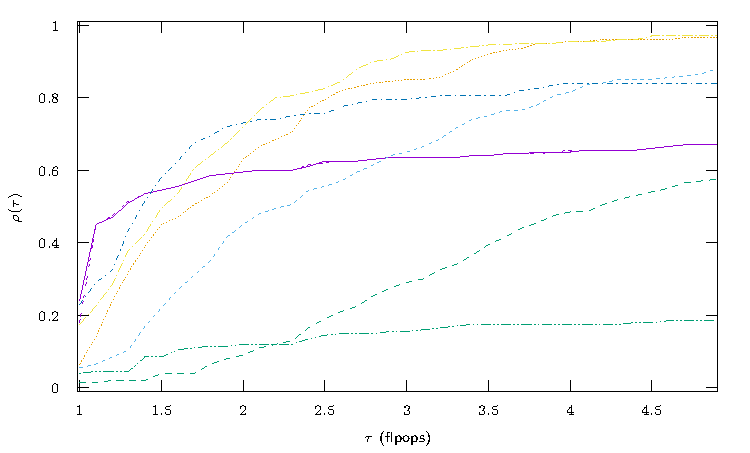
\includegraphics[width=\widthfigure\textwidth]{../figure/PSOR/flpops/profile-Capsules.pdf}\hspace{-3cm} 
    
\includegraphics[width=\widthfigure\textwidth]{../figure/PSOR/flpops//profile-Capsules_legend.pdf}
  }
 \subfigure[KaplasTower $tol = 10^{-8}, timeout=100s$]{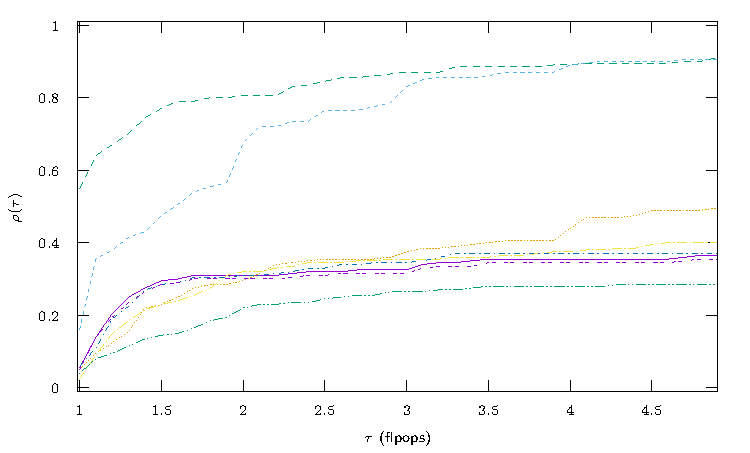
\includegraphics[width=\widthfigure\textwidth]{../figure/PSOR/flpops/profile-KaplasTower.pdf}\hspace{-3cm} 
    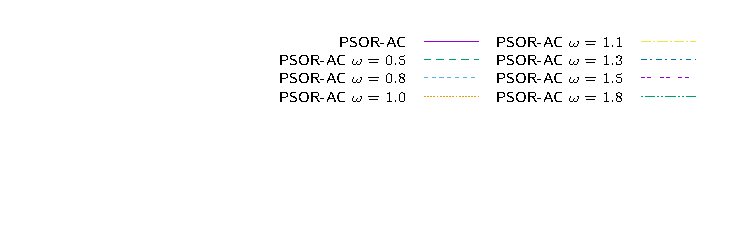
\includegraphics[width=\widthfigure\textwidth]{../figure/PSOR/flpops//profile-KaplasTower_legend.pdf}
  }
  \caption{Effect of relation coefficient $\omega$ in PSOR-AC algorithm($tol_{local} = 10^{-16}$).}
  \label{fig:PSOR/flpops}
\end{figure}

In Figure~\ref{fig:PSOR/flpops}, we study the effect of the relaxation parameter $\omega$ ranging from $[0.5,1.5]$ on the computational time.  Two conclusions can be drawn a) with increasing values of $\omega$, the PSOR algorithm increases its convergence rate as we van observe for $\tau=1$ but b) the robustness of the algorithm is weakened. Indeed, $\tau=15$, we observe that the performance profile is flat and the number of problems solved is higher for valued of $\omega$ around $1$.

To conclude, it is difficult to advice to use PSOR algorithm with $\omega\neq 1$. If it accelerates drastically the rate of convergence of the algorithm for some problems it deteriorates the convergence for other. Further studies would be needed to design self--adaptive schemes for the choice of $\omega$.

\begin{ndrva}
  \item redo this comparison on a set of mixed examples
  \item add some results with $\omega =1.8$ to show that higher values will destroy the convergence.
  \item is it possible to find sizing rule in the literature ?
\end{ndrva}



\subsection{Comparison of PPA-NSN-AC algorithm with respect to  the step-size parameter $\sigma$, $\mu$}

\begin{figure}
  \centering
  \subfigure{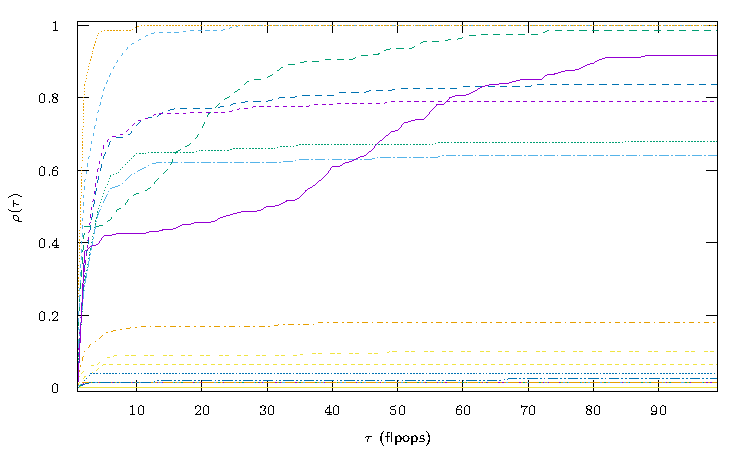
\includegraphics[width=\widthfigure\textwidth]{../figure/PROX/Parameters/flpops//profile-Capsules.pdf} \hspace{-3cm} 
    
\includegraphics[width=\widthfigure\textwidth]{../figure/PROX/Parameters/flpops//profile-Capsules_legend.pdf}
  }
  \subfigure{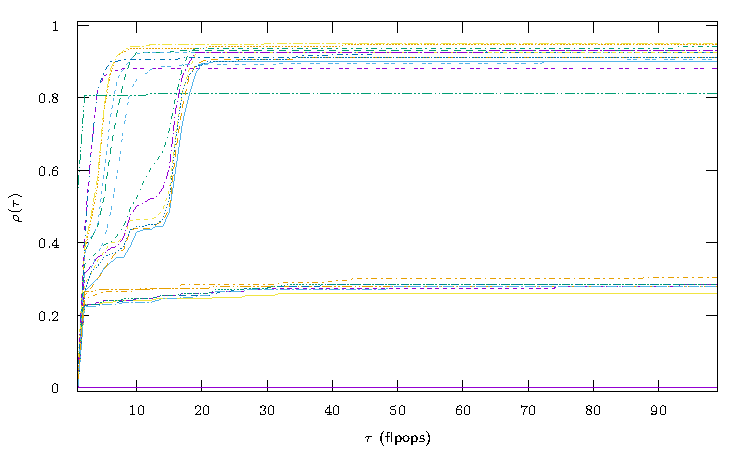
\includegraphics[width=\widthfigure\textwidth]{../figure/PROX/Parameters/flpops/profile-KaplasTower.pdf} \hspace{-3cm} 
    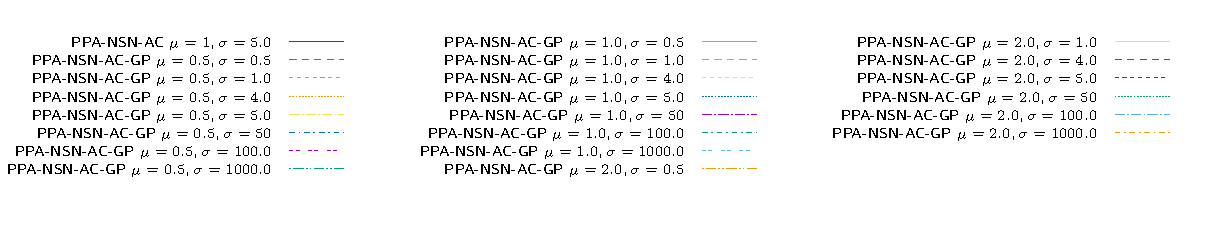
\includegraphics[width=\widthfigure\textwidth]{../figure/PROX/Parameters/flpops//profile-KaplasTower_legend.pdf}
  }
  \caption{Effect of the step-size parameter $\sigma$, $\mu$ in PPA-NSN-AC algorithm}
  \label{fig:profile-Capsules-reduced-PPA-NSN-AC-1_10-time}
\end{figure}

\begin{ndrva}
  \item redo this comparison on a set of mixed examples 
  \item add some results with $\nu < 1 $
\end{ndrva}


\section{Comparison of different families of solvers.}


% \subsection{Rigid bodies applications}
% \begin{figure}
%   \centering
%   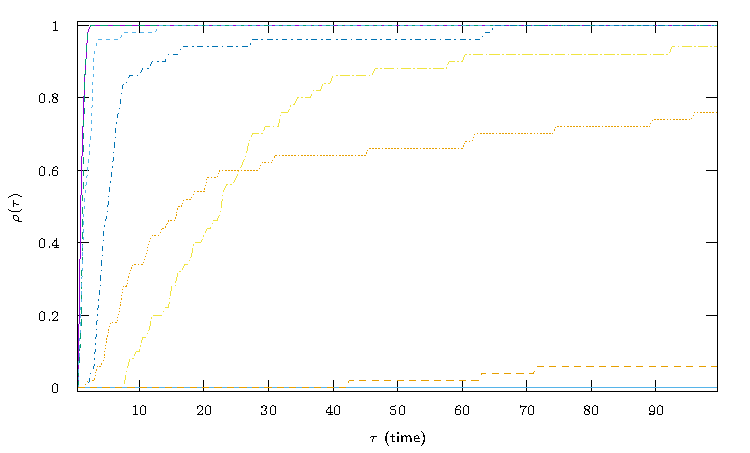
\includegraphics[width=\widthfigure\textwidth]{../figure/profile-LMGC_Bridge_PR-time_0_100.pdf}
%   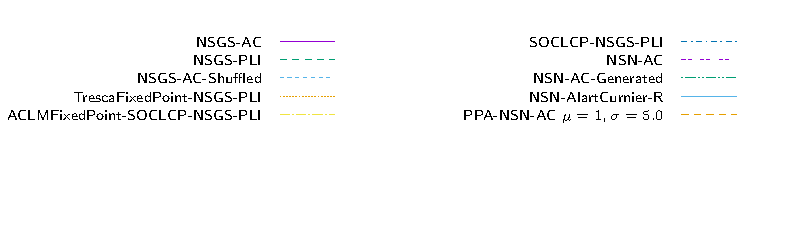
\includegraphics[width=\widthfigure\textwidth]{../figure/profile-LMGC_Bridge_PR_legend-time_0_100.pdf}
%   \caption{Bridge\_PR tests. $timeout=50s, tol = 10^{[-4} $ performance (time). }
%   \label{fig:profile-LMGC_Bridge_PR-time}
% \end{figure}



% \subsection{Finite Element applications}

% \begin{figure}
%   \centering
%   \includegraphics[width=\widthfigure\textwidth]{../figure/profile-LMGC_Cubes_H8-time_0_100.pdf}
%   \includegraphics[width=\widthfigure\textwidth]{../figure/profile-LMGC_Cubes_H8-time_0_5000.pdf}
%   \includegraphics[width=\widthfigure\textwidth]{../figure/profile-LMGC_Cubes_H8_legend-time.pdf}
%   \caption{Cubes H8\_5 tests. $timeout=50s $ performance (time). }
%   \label{fig:profile-LMGC_Cubes_H8-time}
% \end{figure}

% \begin{figure}
%   \centering
%   \includegraphics[width=\widthfigure\textwidth]{../figure/profile-LMGC_Cubes_H8-time_0_100.pdf}
%   \includegraphics[width=\widthfigure\textwidth]{../figure/profile-LMGC_Cubes_H8_legend-time.pdf}
%   \caption{Cubes H8\_20 tests. $timeout=50s $ performance (time). }
%   \label{fig:profile-LMGC_Cubes_H8-time}
% \end{figure}


\subsection{CPU and memory efforts for a given tolerance}

Analyze the quickest one and the more robust one.

\subsection{Analyze reached accuracy for a given time}



\addcontentsline{toc}{section}{References}
\bibliographystyle{plainnat}
\bibliography{./biblio/String,./biblio/NonSmooth,./biblio/Math,./biblio/Multibody,./biblio/Fem.bib,./biblio/Dae.bib,./biblio/Meca,./biblio/AnaNum.bib,./biblio/Math-Impact,./biblio/Contact,./biblio/Optim,./biblio/Cp}
%\bibliography{biblio-extract}



%%% Local Variables: 
%%% mode: latex
%%% TeX-master: "rr"
%%% End: 
